% Options for packages loaded elsewhere
\PassOptionsToPackage{unicode}{hyperref}
\PassOptionsToPackage{hyphens}{url}
%
\documentclass[
]{article}
\usepackage{lmodern}
\usepackage{amssymb,amsmath}
\usepackage{ifxetex,ifluatex}
\ifnum 0\ifxetex 1\fi\ifluatex 1\fi=0 % if pdftex
  \usepackage[T1]{fontenc}
  \usepackage[utf8]{inputenc}
  \usepackage{textcomp} % provide euro and other symbols
\else % if luatex or xetex
  \usepackage{unicode-math}
  \defaultfontfeatures{Scale=MatchLowercase}
  \defaultfontfeatures[\rmfamily]{Ligatures=TeX,Scale=1}
\fi
% Use upquote if available, for straight quotes in verbatim environments
\IfFileExists{upquote.sty}{\usepackage{upquote}}{}
\IfFileExists{microtype.sty}{% use microtype if available
  \usepackage[]{microtype}
  \UseMicrotypeSet[protrusion]{basicmath} % disable protrusion for tt fonts
}{}
\makeatletter
\@ifundefined{KOMAClassName}{% if non-KOMA class
  \IfFileExists{parskip.sty}{%
    \usepackage{parskip}
  }{% else
    \setlength{\parindent}{0pt}
    \setlength{\parskip}{6pt plus 2pt minus 1pt}}
}{% if KOMA class
  \KOMAoptions{parskip=half}}
\makeatother
\usepackage{xcolor}
\IfFileExists{xurl.sty}{\usepackage{xurl}}{} % add URL line breaks if available
\IfFileExists{bookmark.sty}{\usepackage{bookmark}}{\usepackage{hyperref}}
\hypersetup{
  pdftitle={R Notebook for the cystectomy study},
  pdfauthor={Pascal Jerney},
  hidelinks,
  pdfcreator={LaTeX via pandoc}}
\urlstyle{same} % disable monospaced font for URLs
\usepackage[margin=1in]{geometry}
\usepackage{longtable,booktabs}
% Correct order of tables after \paragraph or \subparagraph
\usepackage{etoolbox}
\makeatletter
\patchcmd\longtable{\par}{\if@noskipsec\mbox{}\fi\par}{}{}
\makeatother
% Allow footnotes in longtable head/foot
\IfFileExists{footnotehyper.sty}{\usepackage{footnotehyper}}{\usepackage{footnote}}
\makesavenoteenv{longtable}
\usepackage{graphicx,grffile}
\makeatletter
\def\maxwidth{\ifdim\Gin@nat@width>\linewidth\linewidth\else\Gin@nat@width\fi}
\def\maxheight{\ifdim\Gin@nat@height>\textheight\textheight\else\Gin@nat@height\fi}
\makeatother
% Scale images if necessary, so that they will not overflow the page
% margins by default, and it is still possible to overwrite the defaults
% using explicit options in \includegraphics[width, height, ...]{}
\setkeys{Gin}{width=\maxwidth,height=\maxheight,keepaspectratio}
% Set default figure placement to htbp
\makeatletter
\def\fps@figure{htbp}
\makeatother
\setlength{\emergencystretch}{3em} % prevent overfull lines
\providecommand{\tightlist}{%
  \setlength{\itemsep}{0pt}\setlength{\parskip}{0pt}}
\setcounter{secnumdepth}{5}

\title{R Notebook for the cystectomy study}
\author{Pascal Jerney}
\date{22nd May 2020}

\begin{document}
\maketitle

\begin{verbatim}
## Loading required package: pacman
\end{verbatim}

\hypertarget{index}{%
\section{Index}\label{index}}

Welcome to the notebook!

\hypertarget{table-1}{%
\subsection{Table 1}\label{table-1}}

\begin{tabular}{l|l|l|l|l}
\hline
  & FALSE & TRUE & p & test\\
\hline
n & 798 & 369 &  & \\
\hline
blood\_loss\_ml (median [IQR]) & 900.00 [700.00, 1245.00] & 1400.00 [1000.00, 2100.00] & <0.001 & nonnorm\\
\hline
blood\_loss\_ratio (median [IQR]) & 0.19 [0.14, 0.26] & 0.31 [0.22, 0.42] & <0.001 & nonnorm\\
\hline
oak = TRUE (\%) & 23 (2.9) & 21 (5.7) & 0.029 & \\
\hline
tcaggr = TRUE (\%) & 87 (10.9) & 40 (10.8) & 1.000 & \\
\hline
preop\_hb (median [IQR]) & 135.00 [123.00, 145.00] & 120.00 [104.00, 130.00] & <0.001 & nonnorm\\
\hline
preop\_tc (median [IQR]) & 251.50 [211.00, 309.00] & 267.00 [214.00, 339.00] & 0.003 & nonnorm\\
\hline
bmi (median [IQR]) & 25.56 [22.86, 28.72] & 25.39 [22.71, 28.52] & 0.701 & nonnorm\\
\hline
age (median [IQR]) & 67.08 [59.21, 74.29] & 71.03 [64.04, 77.48] & <0.001 & nonnorm\\
\hline
cci\_5plus (\%) &  &  & <0.001 & \\
\hline
0 & 304 (38.1) & 106 (28.7) &  & \\
\hline
1 & 131 (16.4) & 48 (13.0) &  & \\
\hline
2 & 181 (22.7) & 89 (24.1) &  & \\
\hline
3 & 98 (12.3) & 56 (15.2) &  & \\
\hline
4 & 55 (6.9) & 37 (10.0) &  & \\
\hline
5 and more & 29 (3.6) & 33 (8.9) &  & \\
\hline
gender = female (\%) & 239 (29.9) & 140 (37.9) & 0.008 & \\
\hline
p\_tumor (\%) &  &  & <0.001 & \\
\hline
0 & 201 (25.2) & 58 (15.7) &  & \\
\hline
1 & 111 (13.9) & 38 (10.3) &  & \\
\hline
2 & 193 (24.2) & 75 (20.3) &  & \\
\hline
3 & 233 (29.2) & 129 (35.0) &  & \\
\hline
4 & 60 (7.5) & 69 (18.7) &  & \\
\hline
p\_nodes (\%) &  &  & 0.002 & \\
\hline
0 & 631 (79.1) & 266 (72.1) &  & \\
\hline
1 & 73 (9.1) & 40 (10.8) &  & \\
\hline
2 & 69 (8.6) & 57 (15.4) &  & \\
\hline
3 & 25 (3.1) & 6 (1.6) &  & \\
\hline
op\_year (\%) &  &  & <0.001 & \\
\hline
2000 & 14 (1.8) & 35 (9.5) &  & \\
\hline
2001 & 25 (3.1) & 29 (7.9) &  & \\
\hline
2002 & 27 (3.4) & 19 (5.1) &  & \\
\hline
2003 & 54 (6.8) & 21 (5.7) &  & \\
\hline
2004 & 43 (5.4) & 26 (7.0) &  & \\
\hline
2005 & 31 (3.9) & 17 (4.6) &  & \\
\hline
2006 & 30 (3.8) & 26 (7.0) &  & \\
\hline
2007 & 46 (5.8) & 30 (8.1) &  & \\
\hline
2008 & 69 (8.6) & 19 (5.1) &  & \\
\hline
2009 & 47 (5.9) & 18 (4.9) &  & \\
\hline
2010 & 70 (8.8) & 22 (6.0) &  & \\
\hline
2011 & 69 (8.6) & 22 (6.0) &  & \\
\hline
2012 & 52 (6.5) & 29 (7.9) &  & \\
\hline
2013 & 74 (9.3) & 18 (4.9) &  & \\
\hline
2014 & 64 (8.0) & 15 (4.1) &  & \\
\hline
2015 & 53 (6.6) & 12 (3.3) &  & \\
\hline
2016 & 30 (3.8) & 11 (3.0) &  & \\
\hline
op\_duration\_min (median [IQR]) & 390.00 [345.00, 425.75] & 408.00 [350.00, 451.00] & <0.001 & nonnorm\\
\hline
previous\_op = TRUE (\%) & 326 (40.9) & 161 (43.6) & 0.406 & \\
\hline
norepinephrine = TRUE (\%) & 519 (65.0) & 203 (55.0) & 0.001 & \\
\hline
crystalloids\_mlkgh (median [IQR]) & 4.50 [3.30, 6.01] & 5.30 [3.79, 7.09] & <0.001 & nonnorm\\
\hline
neoadj\_chemo = TRUE (\%) & 101 (12.7) & 75 (20.3) & 0.001 & \\
\hline
\end{tabular}

\hypertarget{prerequisites}{%
\section{Prerequisites}\label{prerequisites}}

\hypertarget{formulas}{%
\subsection{Formulas}\label{formulas}}

\begin{itemize}
\tightlist
\item
  Indexed blood volume\footnote{Lemmens, H. J. M., Bernstein, D. P., \& Brodsky, J. B. (2006). Estimating blood volume in obese and morbidly obese patients. Obesity Surgery, 16(6), 773--776. \url{https://doi.org/10.1381/096089206777346673}}: \(BV_i = \frac{70}{\sqrt{\frac{BMI}{22}}}\)\footnote{\(BV_i\) = Indexed blood volume, \(BMI\) = Body mass index}
\item
  Estimated blood volume: \(BV_e = BV_i \cdot Weight\)\footnote{\(BV_e\) = Estimated blood volume}
\item
  Blood loss ratio: \(BL_r = \frac{BV_e}{BL_a}\)\footnote{\(BL_r\) = Blood loss ratio, \(BL_a\) = Absolute blood loss}
\item
  Standardization method for age and bmi\footnote{Iglewicz, B., \& Hoaglin, D. C. (1993). How to detect and handle outliers. Milwaukee, Wis: ASQC Quality Press.}: \(M_i = \frac{0.6745(x_i - \tilde(x))}{2 \cdot MAD}\)\footnote{\(M_i\) = Modified Z-score, \(\tilde(x)\) = Median of \(x\), \(MAD\) = Median absolute deviation}
\end{itemize}

\hypertarget{results}{%
\section{Results}\label{results}}

\hypertarget{data-plots}{%
\subsection{Data plots}\label{data-plots}}

\begin{center}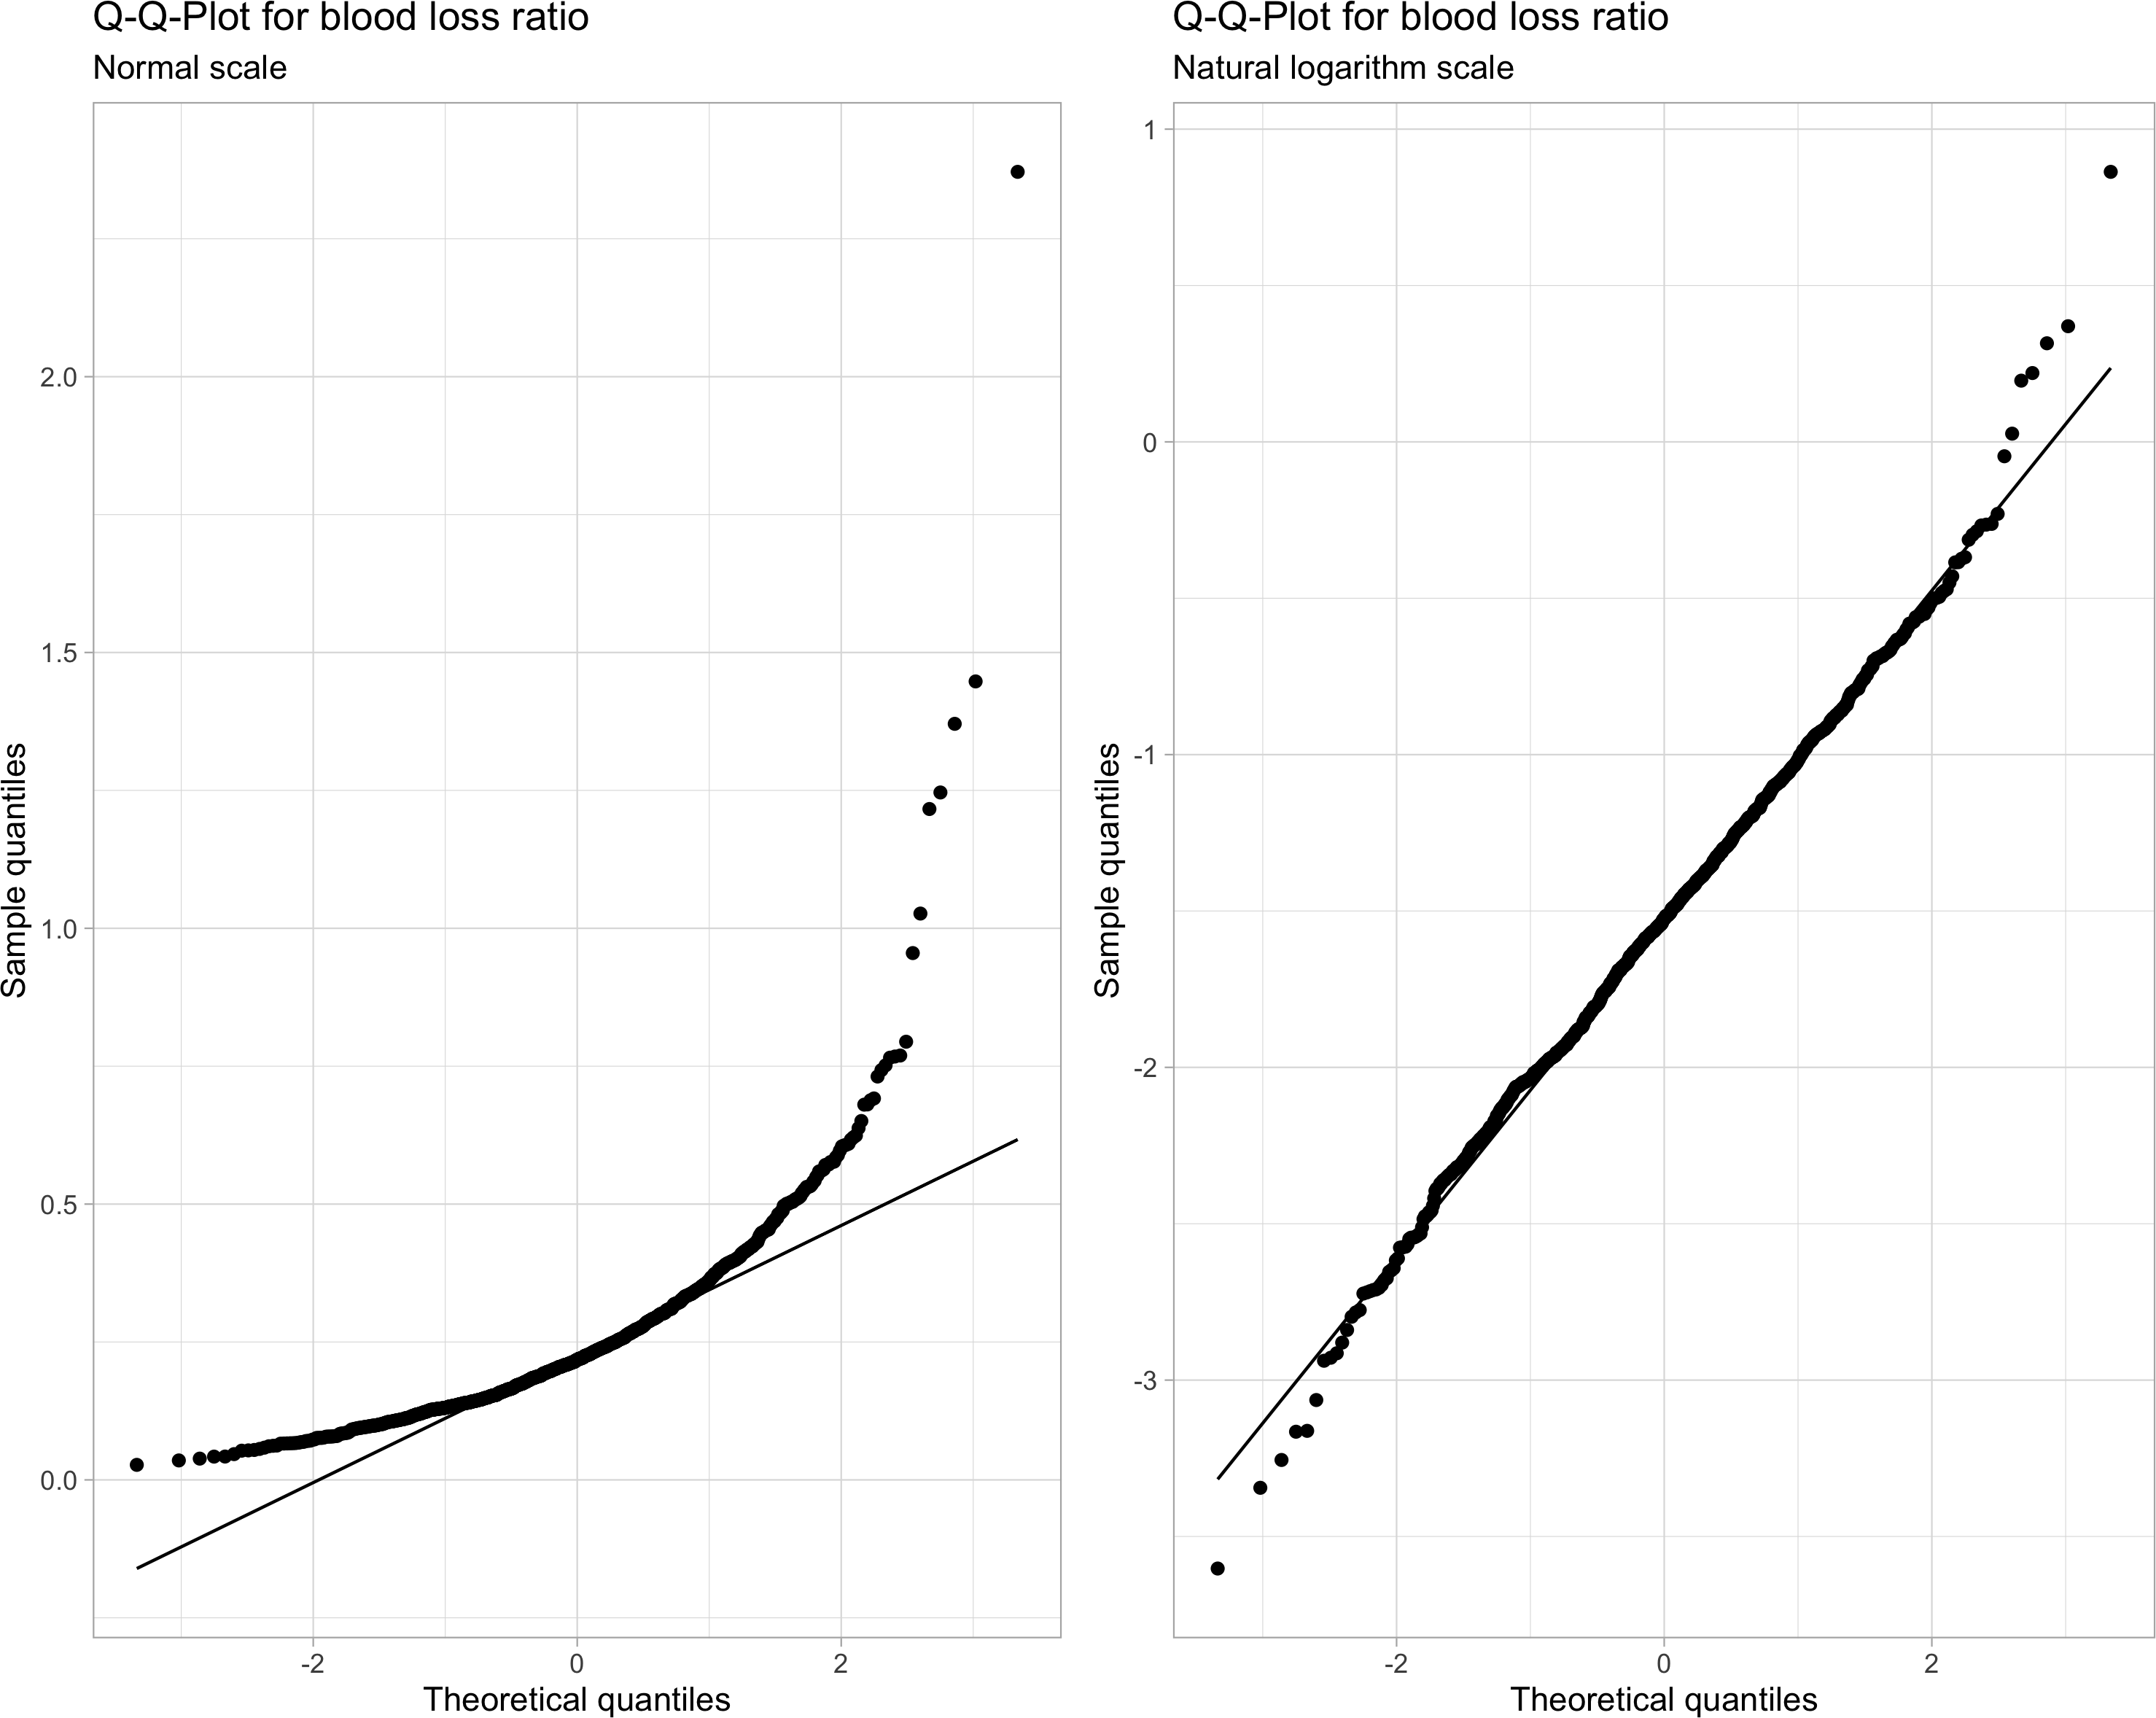
\includegraphics[width=1\linewidth]{notebook_files/figure-latex/data_plots-1} \end{center}

\begin{center}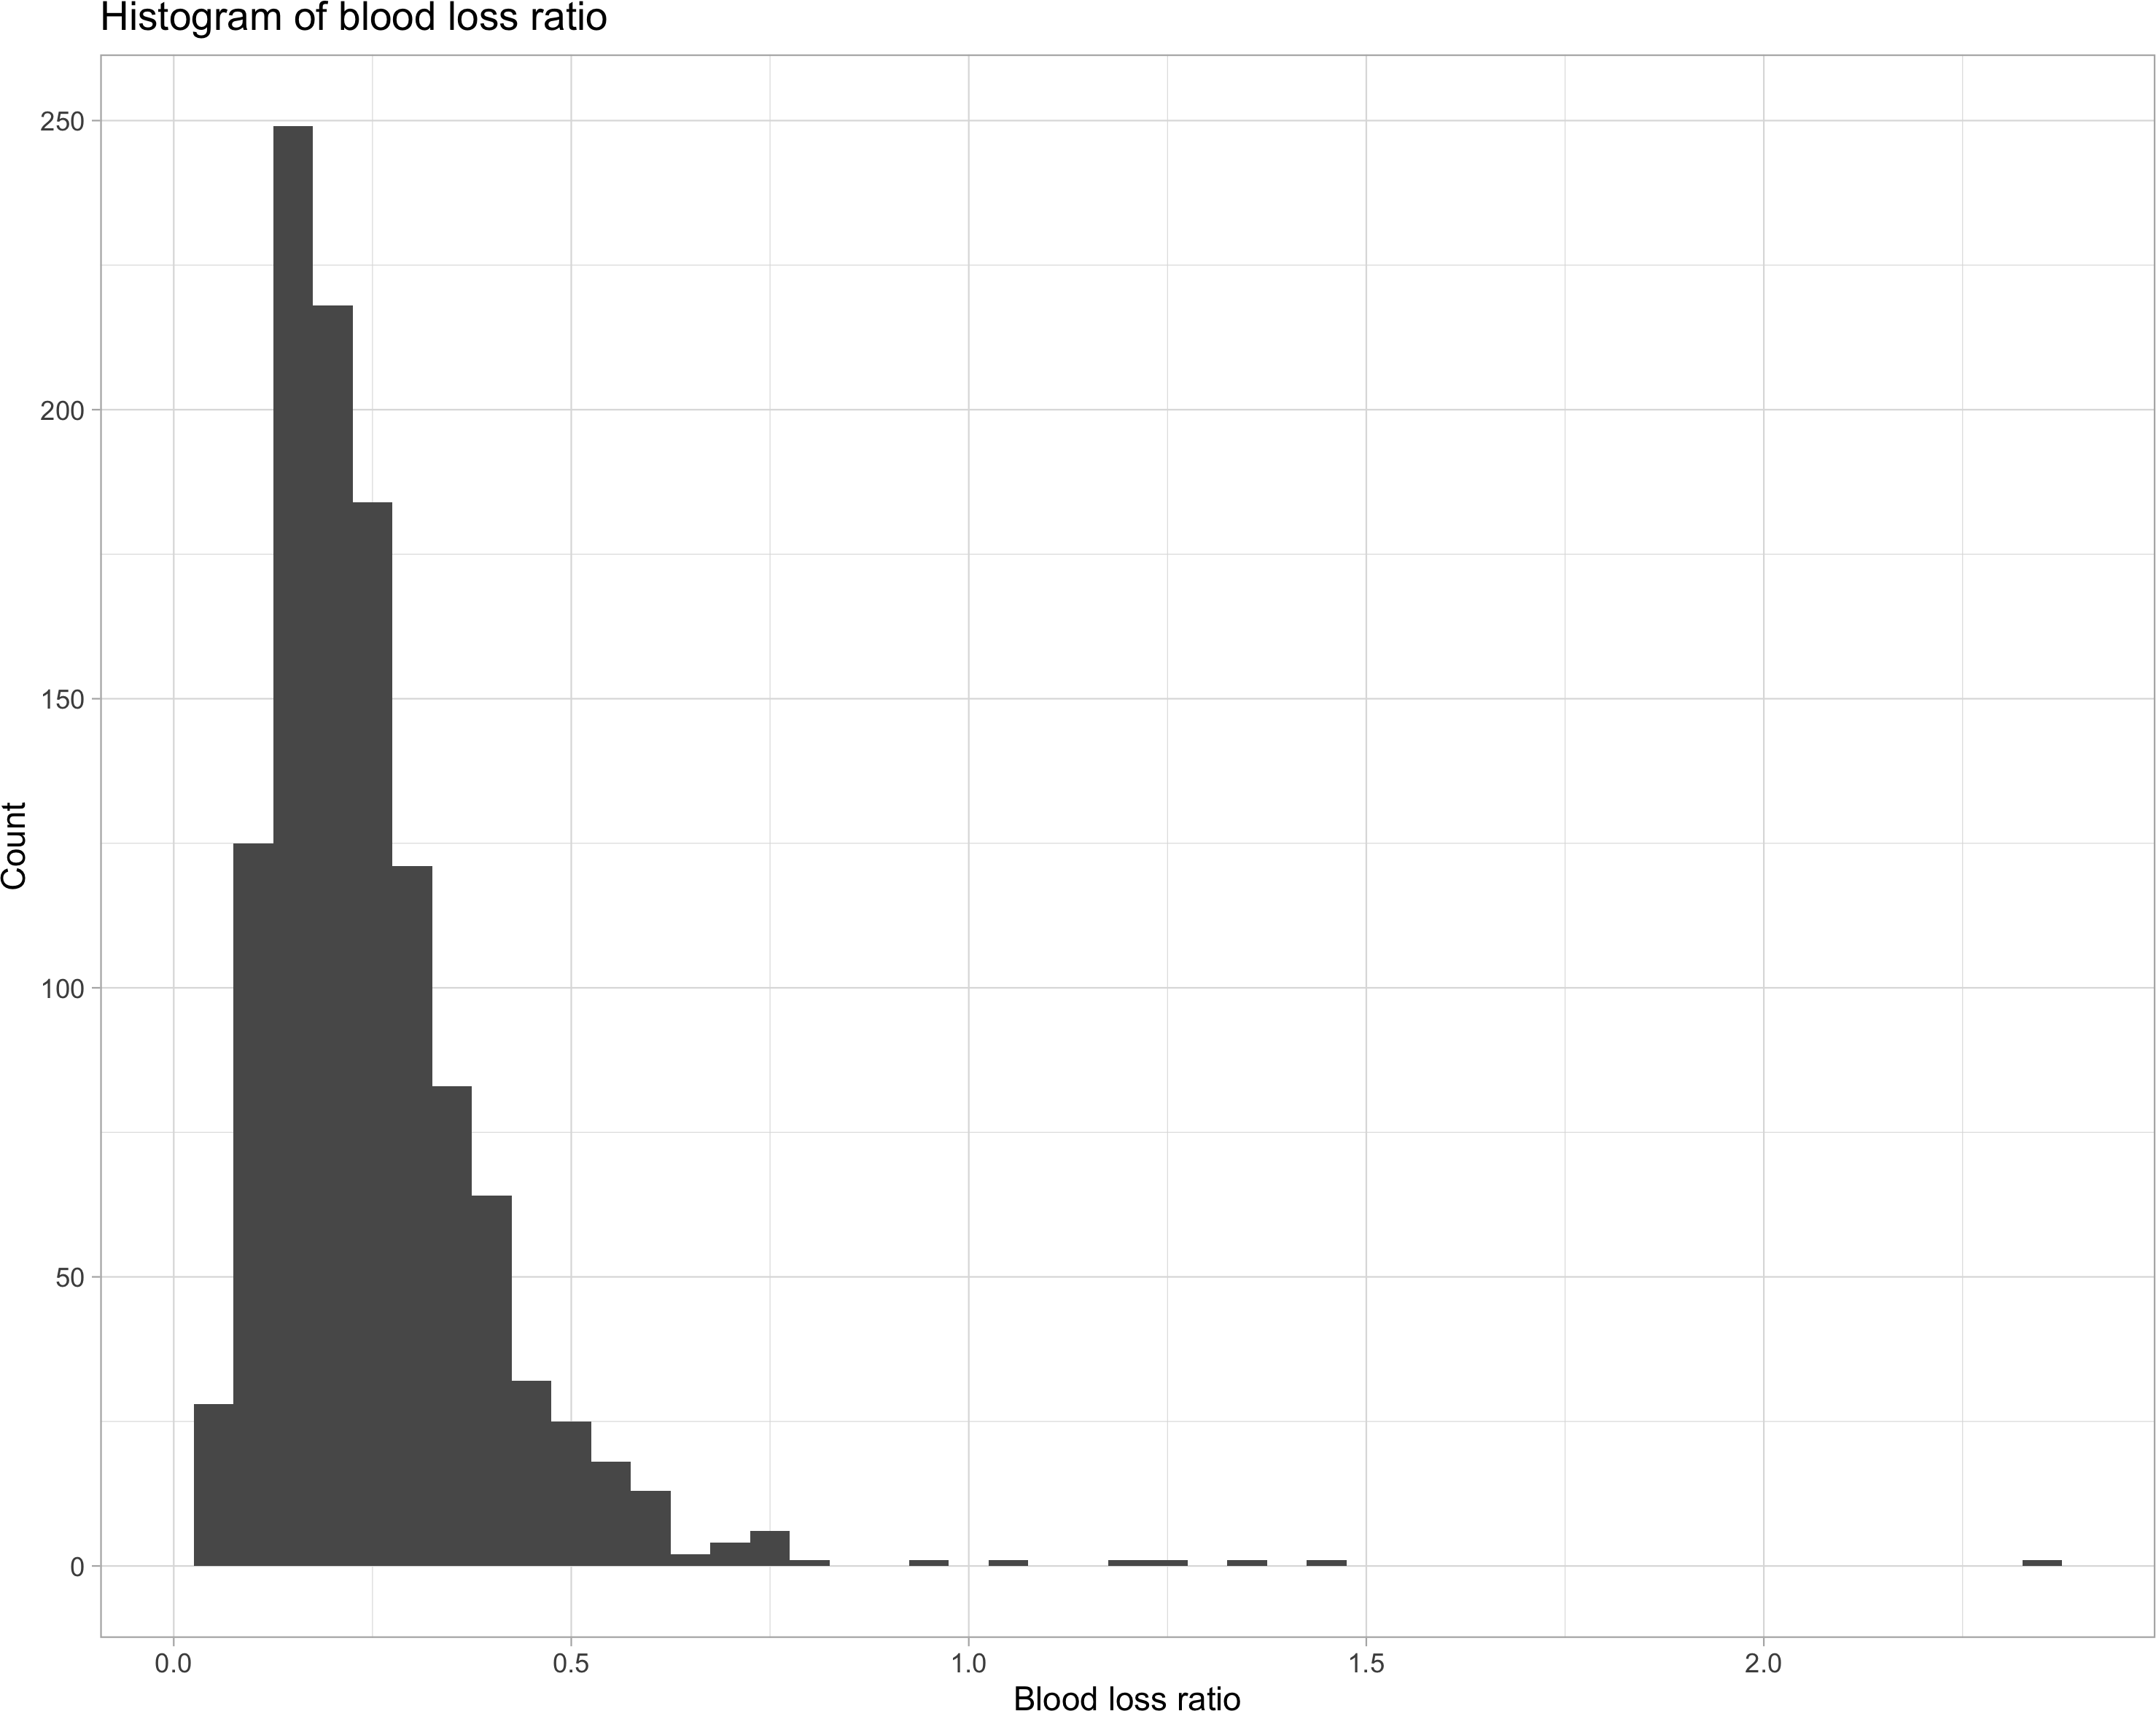
\includegraphics[width=1\linewidth]{notebook_files/figure-latex/data_plots-2} \end{center}

\begin{center}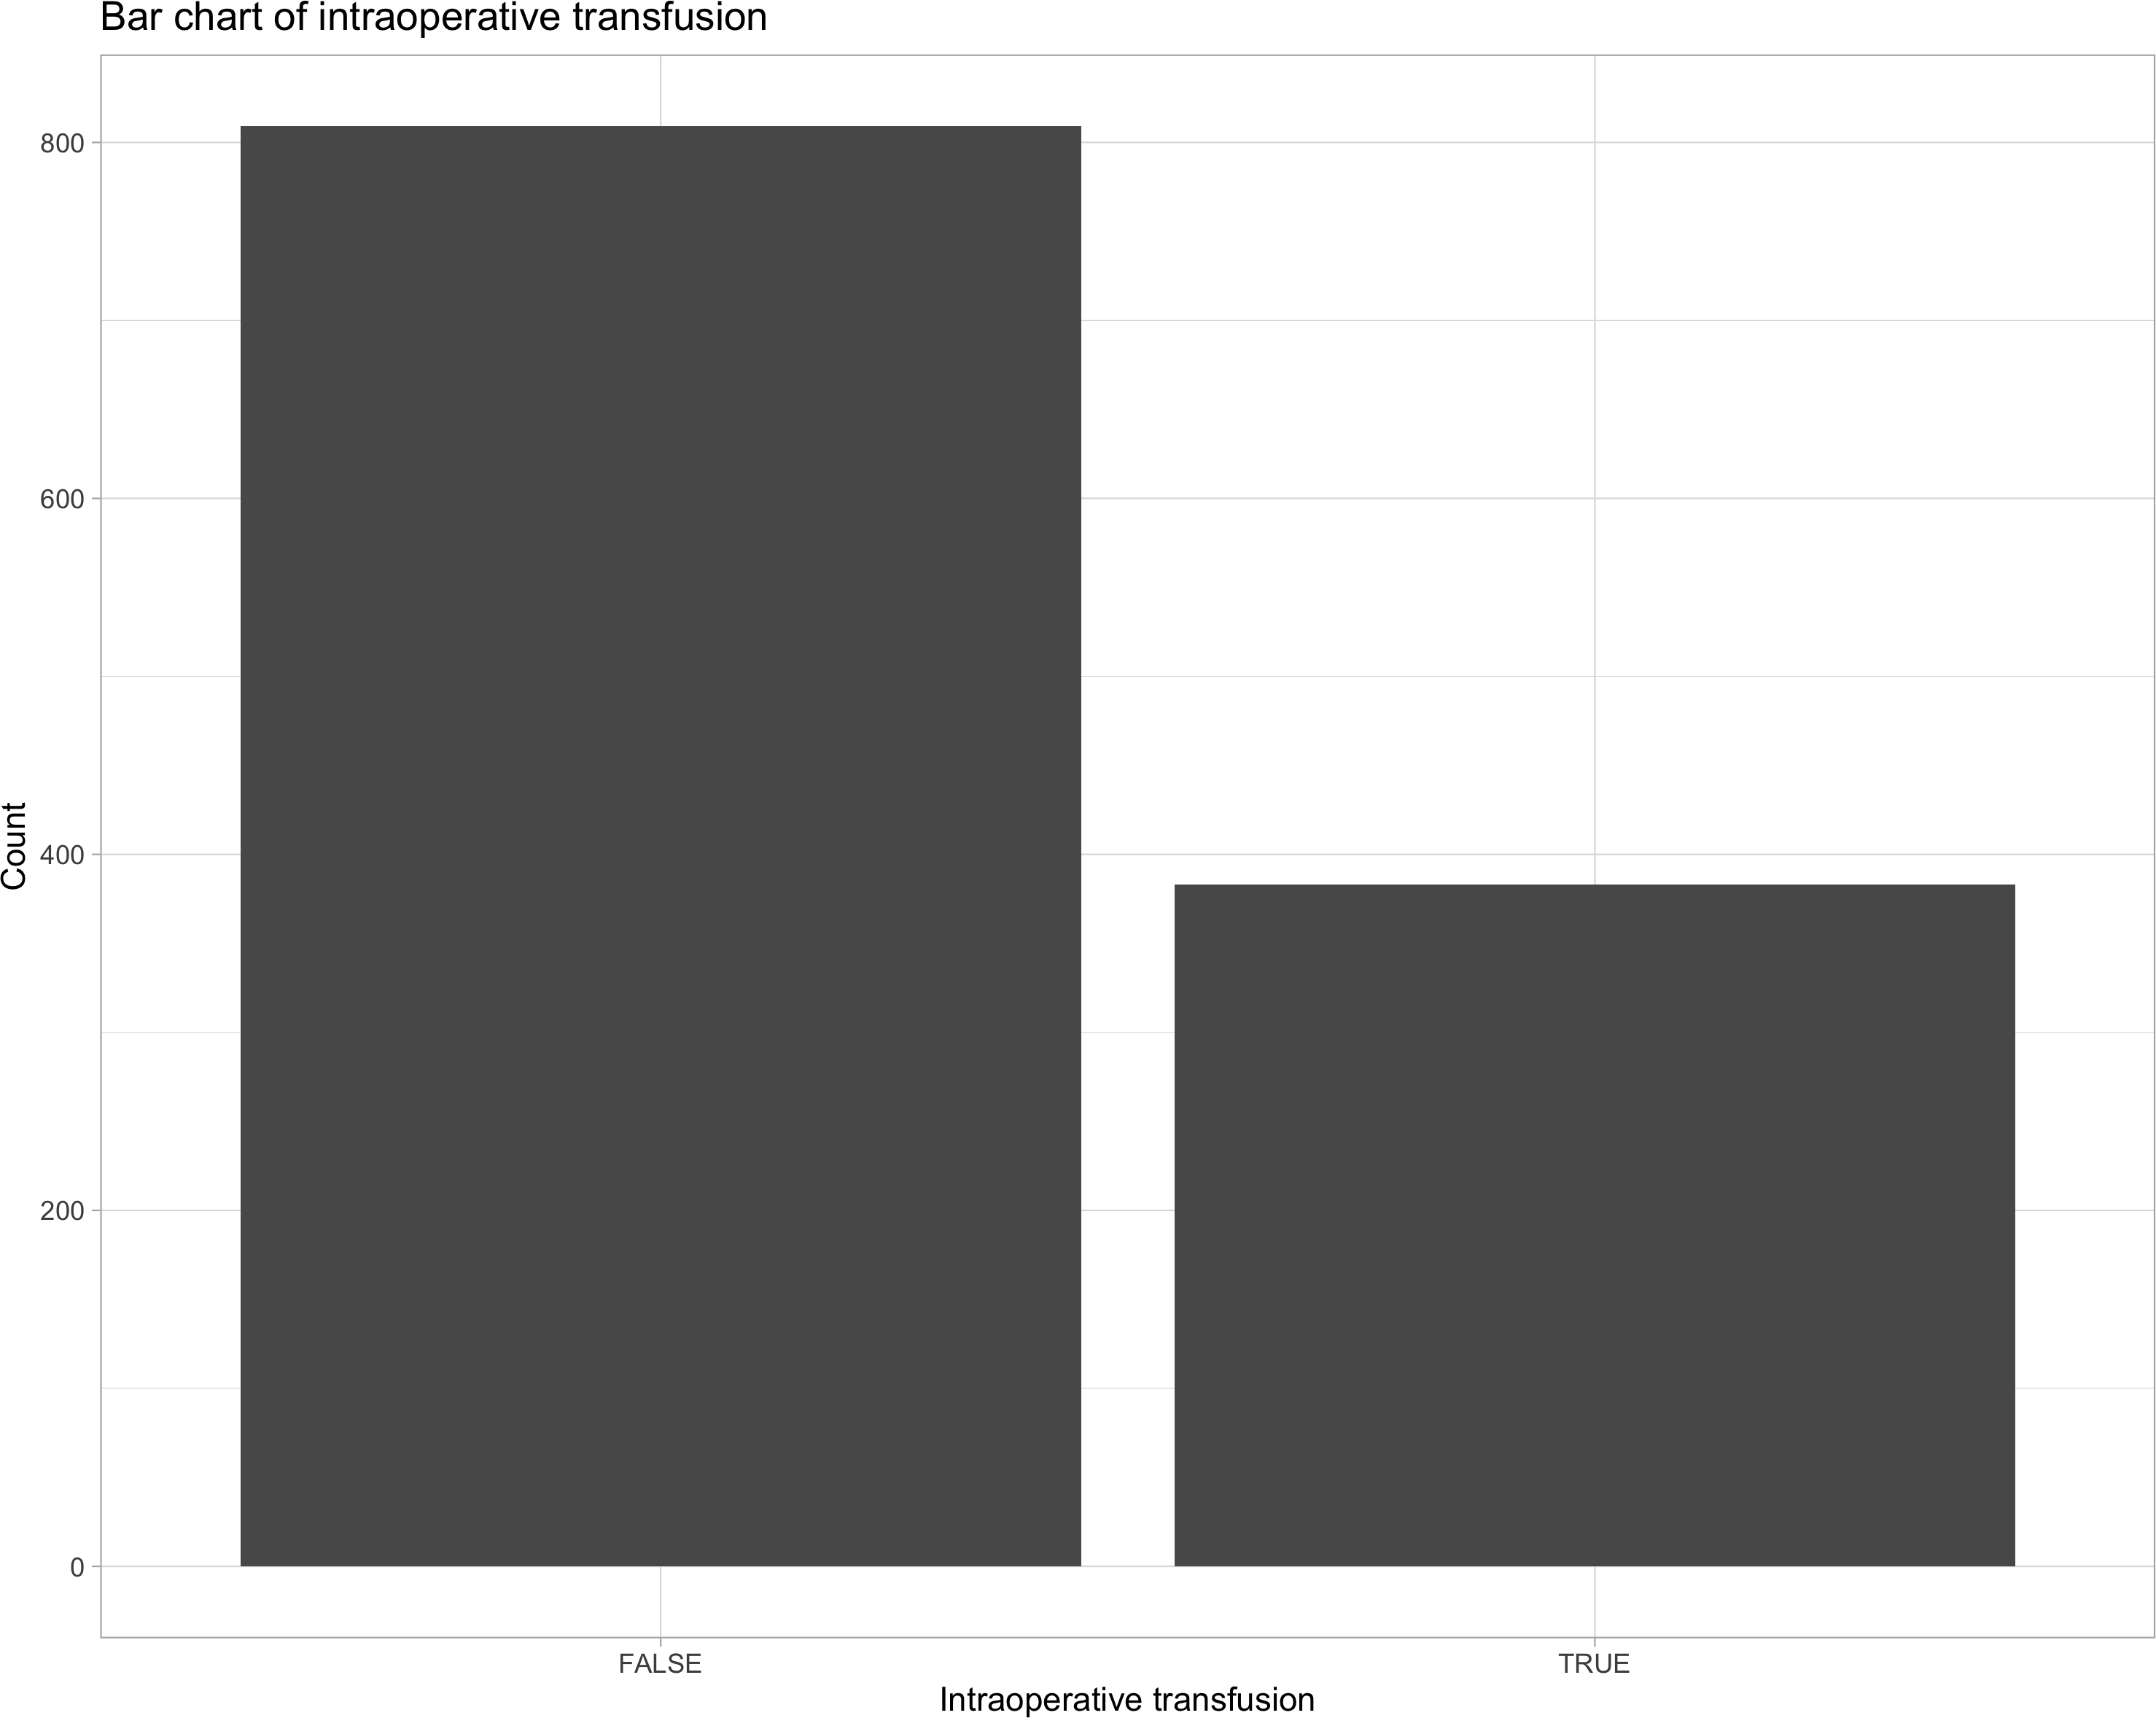
\includegraphics[width=1\linewidth]{notebook_files/figure-latex/data_plots-3} \end{center}

\hypertarget{model-outputs}{%
\subsection{Model outputs}\label{model-outputs}}

\hypertarget{models-with-intraoperative-transfusion-as-response}{%
\subsubsection{Models with intraoperative transfusion as response}\label{models-with-intraoperative-transfusion-as-response}}

\hypertarget{full-model}{%
\paragraph{Full model}\label{full-model}}

\hypertarget{diagnostics}{%
\subparagraph{Diagnostics}\label{diagnostics}}

\begin{verbatim}
#> No divergences to plot.
\end{verbatim}

\begin{center}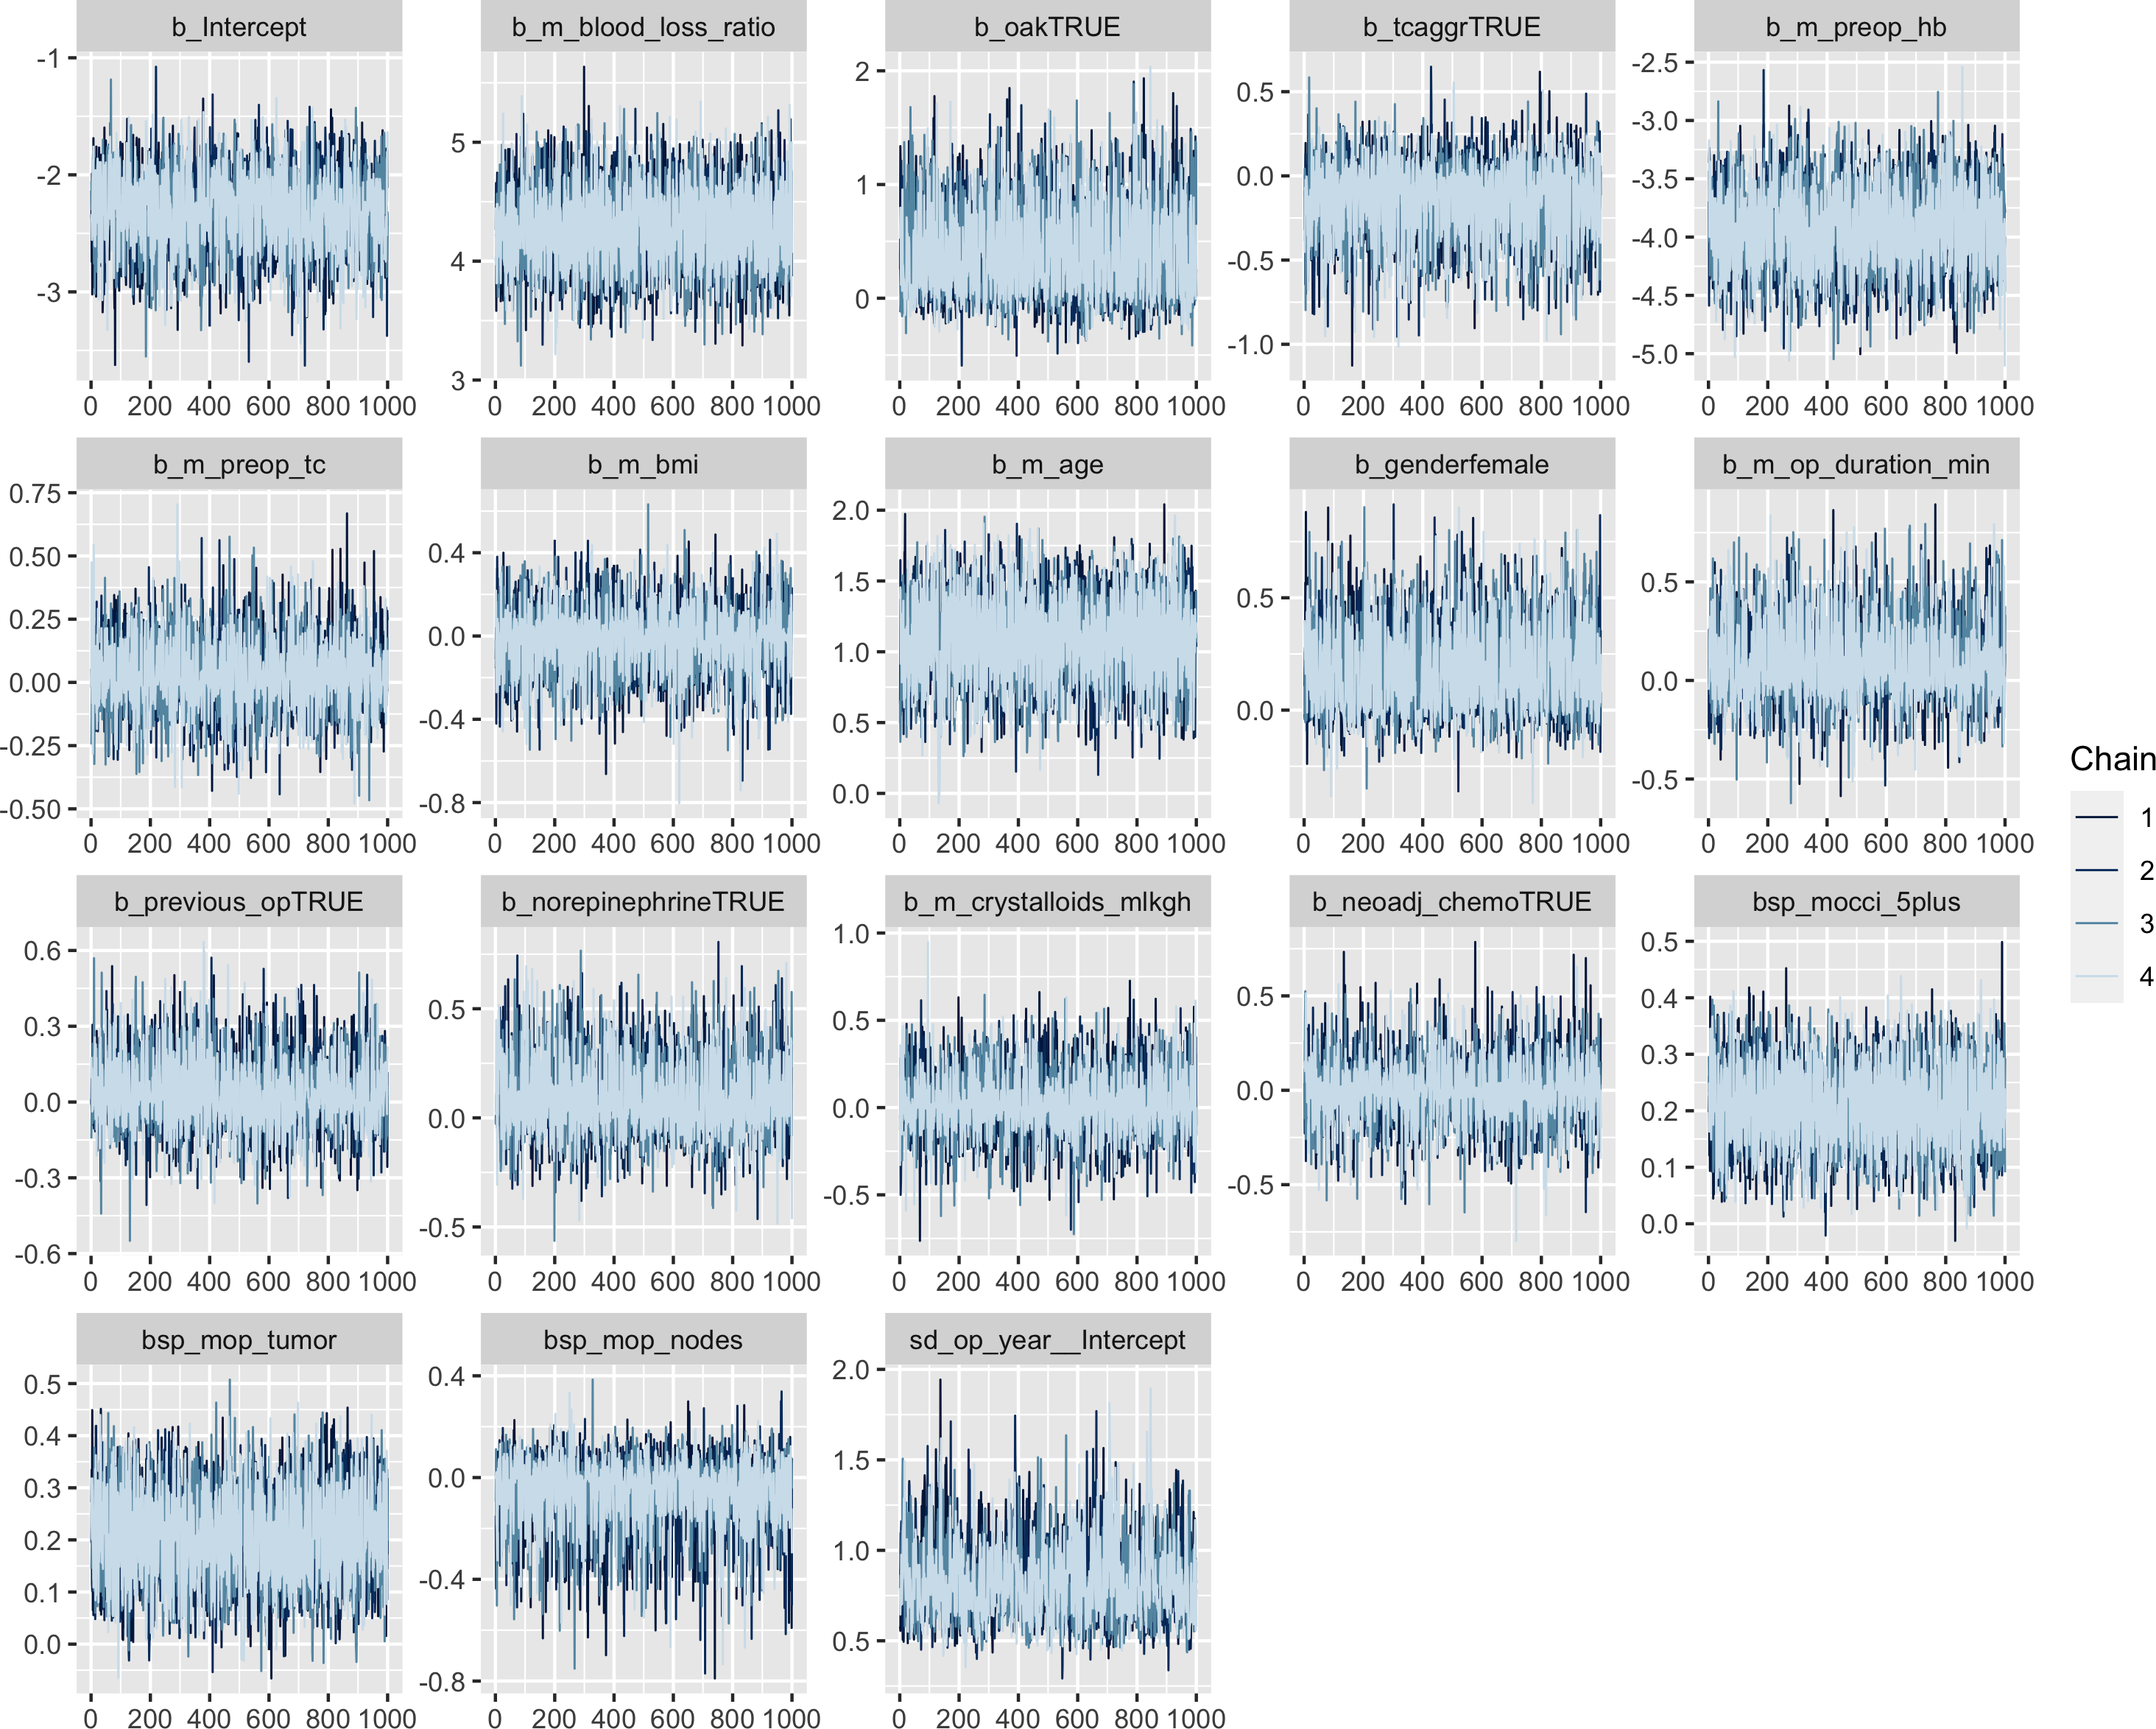
\includegraphics[width=1\linewidth]{notebook_files/figure-latex/model1full_diagnostics-1} \end{center}

\begin{center}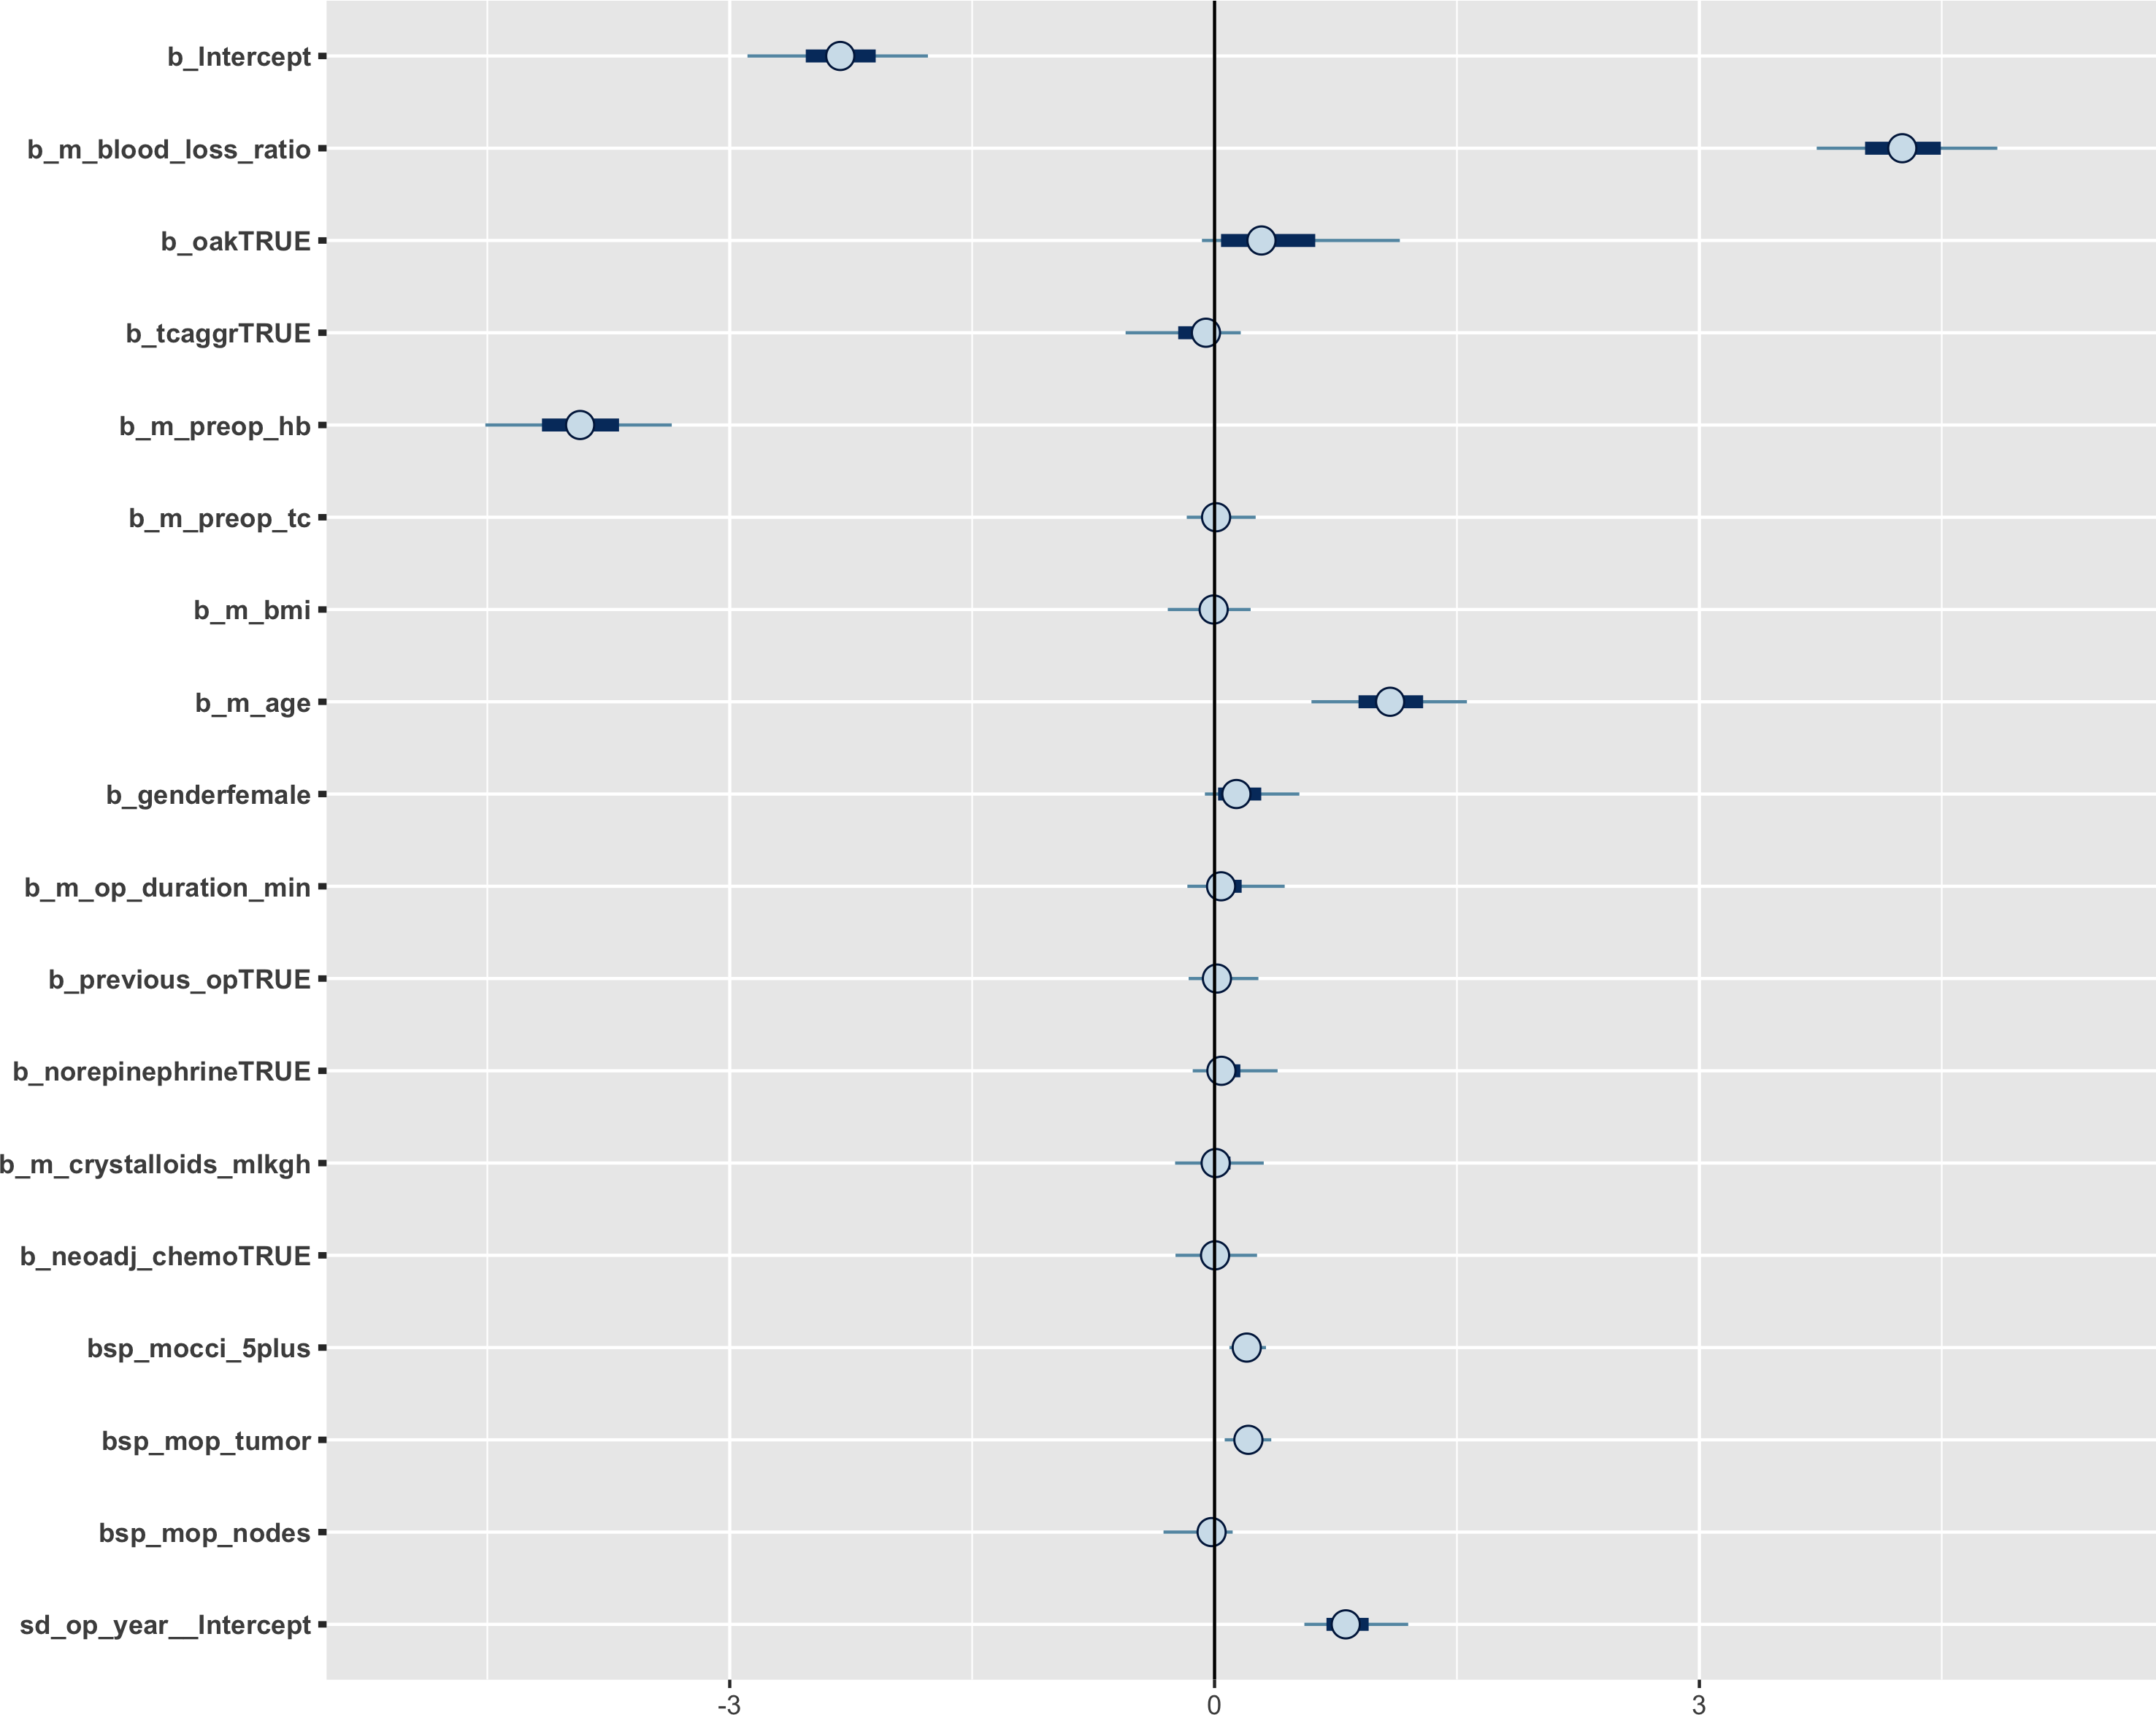
\includegraphics[width=1\linewidth]{notebook_files/figure-latex/model1full_diagnostics-2} \end{center}

\hypertarget{posterior-predictive-check-plot}{%
\subparagraph{Posterior predictive check plot}\label{posterior-predictive-check-plot}}

\begin{verbatim}
#> Using 10 posterior samples for ppc type 'bars' by default.
\end{verbatim}

\begin{center}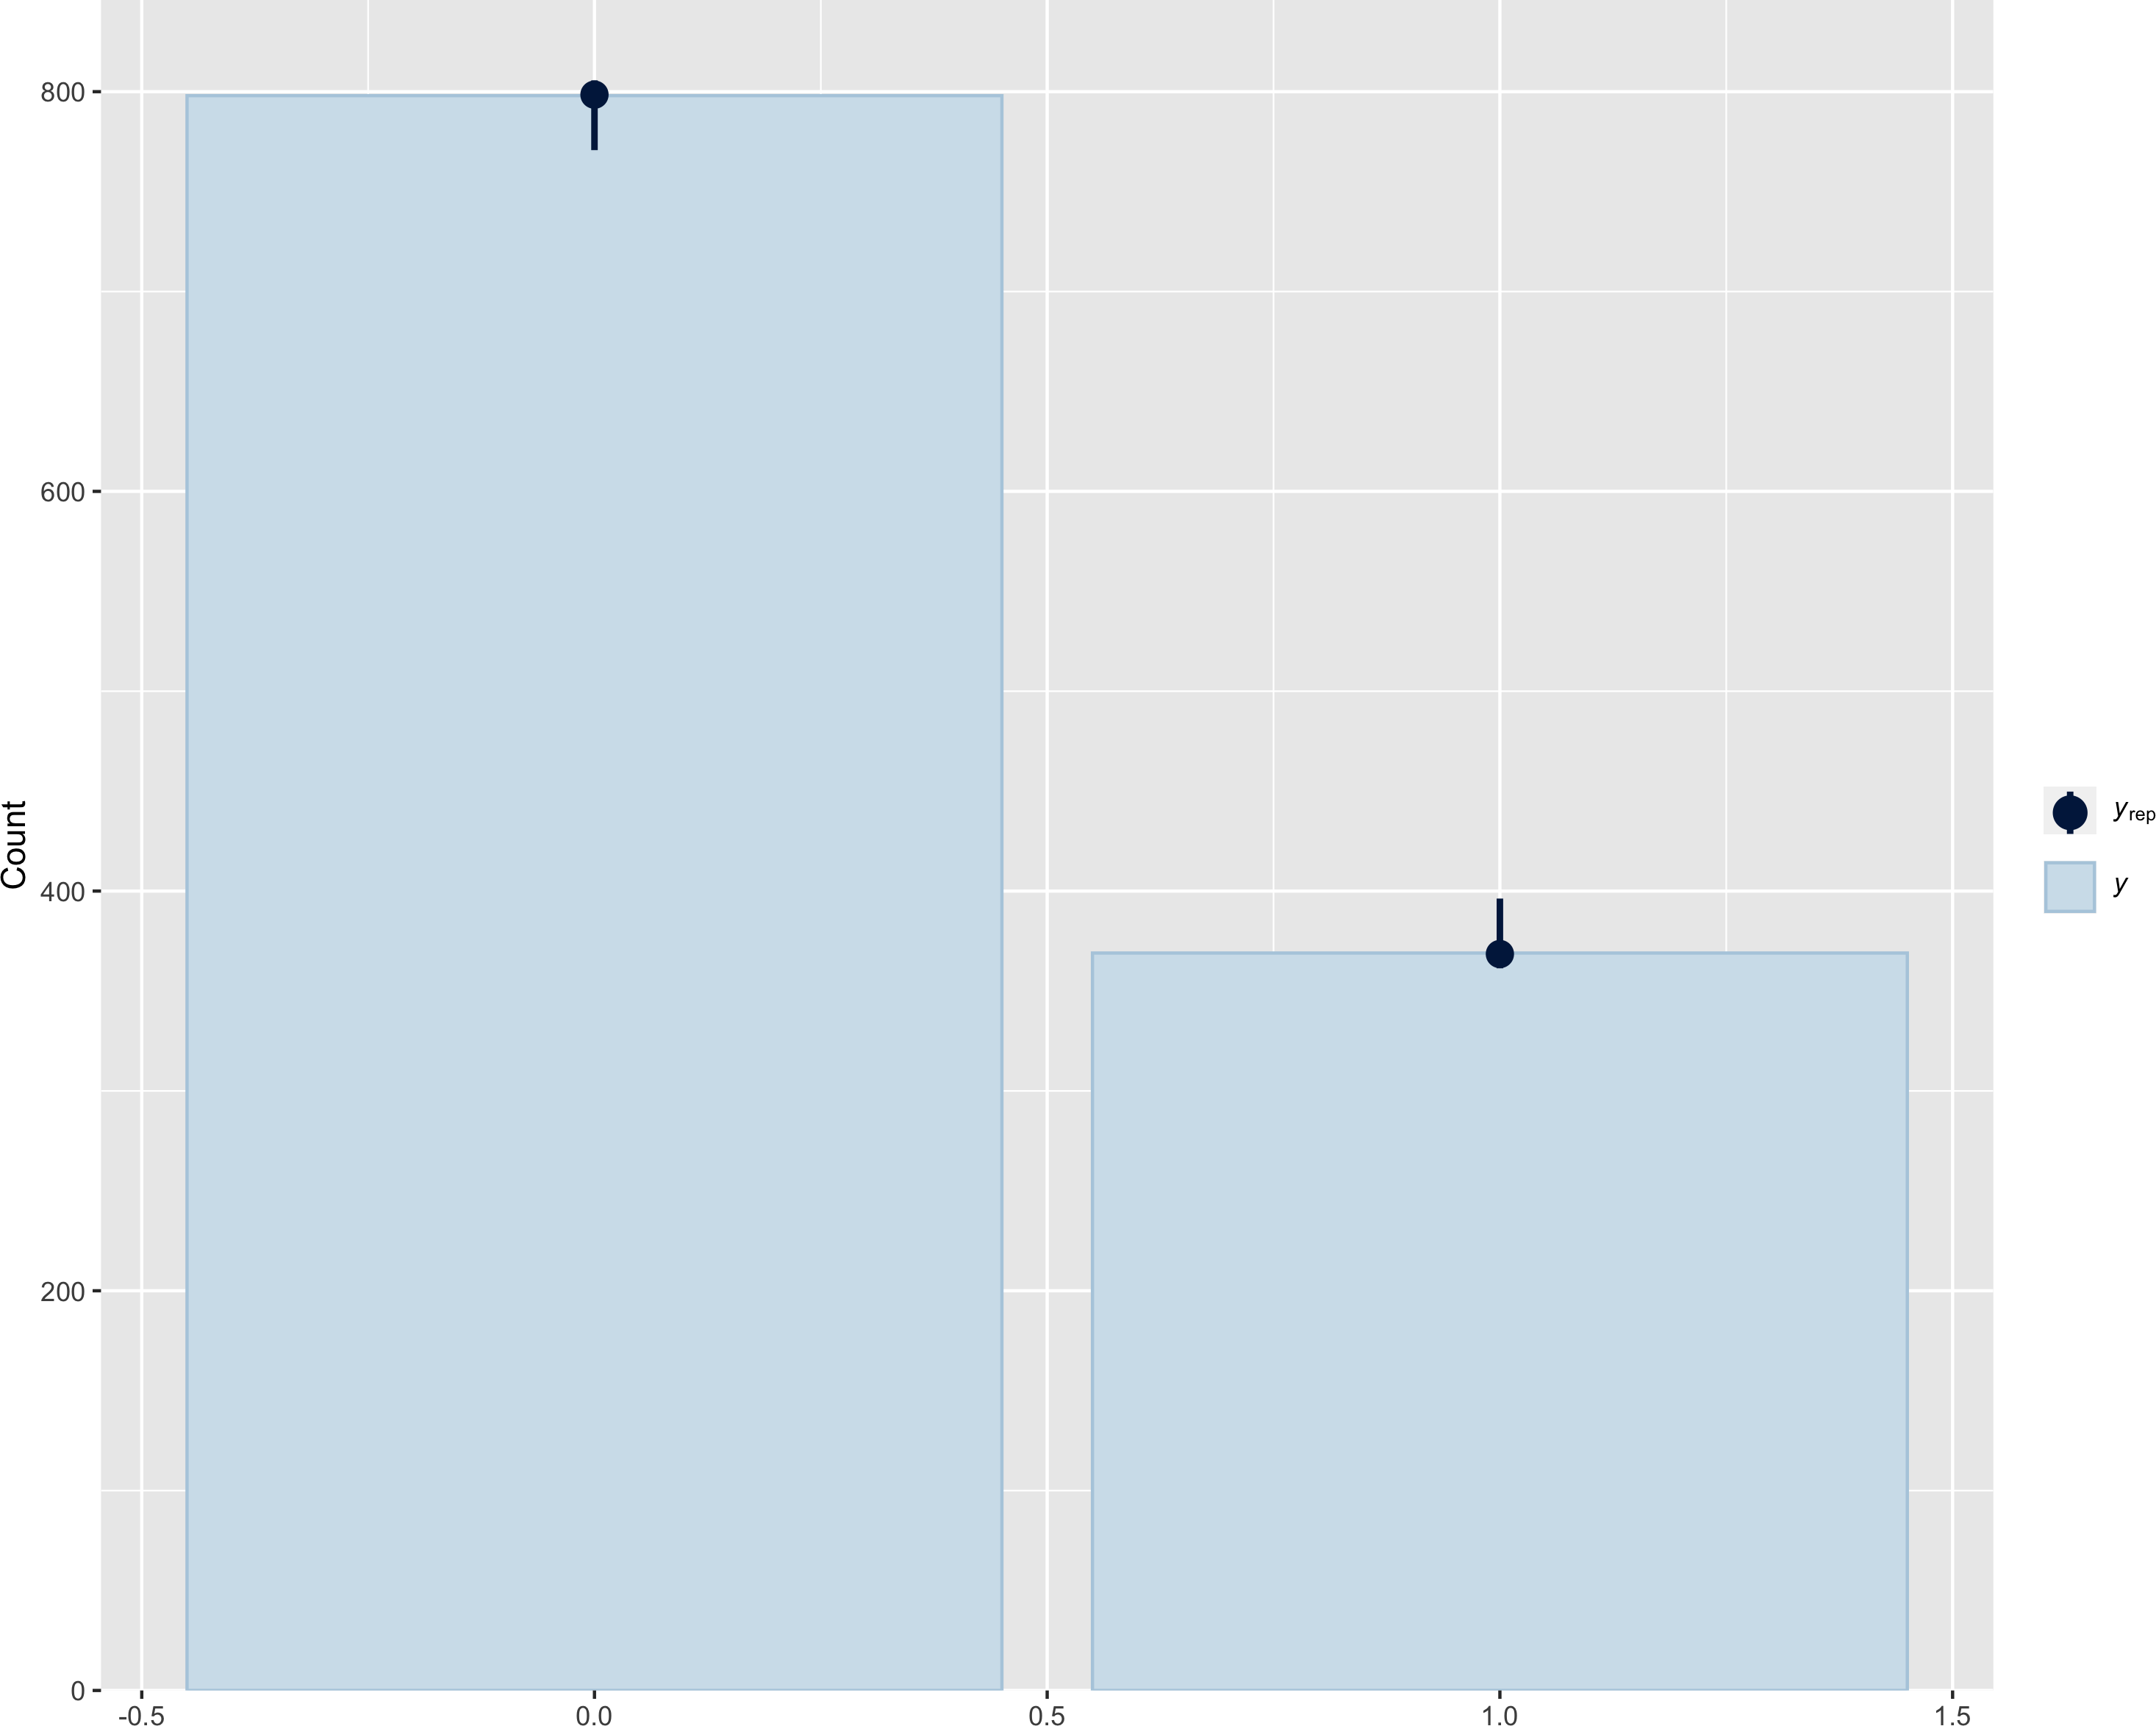
\includegraphics[width=1\linewidth]{notebook_files/figure-latex/model1full_ppcheck-1} \end{center}

\hypertarget{summary}{%
\subparagraph{Summary}\label{summary}}

\begin{longtable}[]{@{}ccccccc@{}}
\caption{Table continues below}\tabularnewline
\toprule
\begin{minipage}[b]{0.09\columnwidth}\centering
~\strut
\end{minipage} & \begin{minipage}[b]{0.25\columnwidth}\centering
Parameter\strut
\end{minipage} & \begin{minipage}[b]{0.11\columnwidth}\centering
Median\strut
\end{minipage} & \begin{minipage}[b]{0.05\columnwidth}\centering
CI\strut
\end{minipage} & \begin{minipage}[b]{0.10\columnwidth}\centering
CI\_low\strut
\end{minipage} & \begin{minipage}[b]{0.10\columnwidth}\centering
CI\_high\strut
\end{minipage} & \begin{minipage}[b]{0.11\columnwidth}\centering
p\_MAP\strut
\end{minipage}\tabularnewline
\midrule
\endfirsthead
\toprule
\begin{minipage}[b]{0.09\columnwidth}\centering
~\strut
\end{minipage} & \begin{minipage}[b]{0.25\columnwidth}\centering
Parameter\strut
\end{minipage} & \begin{minipage}[b]{0.11\columnwidth}\centering
Median\strut
\end{minipage} & \begin{minipage}[b]{0.05\columnwidth}\centering
CI\strut
\end{minipage} & \begin{minipage}[b]{0.10\columnwidth}\centering
CI\_low\strut
\end{minipage} & \begin{minipage}[b]{0.10\columnwidth}\centering
CI\_high\strut
\end{minipage} & \begin{minipage}[b]{0.11\columnwidth}\centering
p\_MAP\strut
\end{minipage}\tabularnewline
\midrule
\endhead
\begin{minipage}[t]{0.09\columnwidth}\centering
\textbf{2}\strut
\end{minipage} & \begin{minipage}[t]{0.25\columnwidth}\centering
b\_Intercept\strut
\end{minipage} & \begin{minipage}[t]{0.11\columnwidth}\centering
-2.301\strut
\end{minipage} & \begin{minipage}[t]{0.05\columnwidth}\centering
95\strut
\end{minipage} & \begin{minipage}[t]{0.10\columnwidth}\centering
-2.964\strut
\end{minipage} & \begin{minipage}[t]{0.10\columnwidth}\centering
-1.682\strut
\end{minipage} & \begin{minipage}[t]{0.11\columnwidth}\centering
0\strut
\end{minipage}\tabularnewline
\begin{minipage}[t]{0.09\columnwidth}\centering
\textbf{4}\strut
\end{minipage} & \begin{minipage}[t]{0.25\columnwidth}\centering
b\_m\_blood\_loss\_ratio\strut
\end{minipage} & \begin{minipage}[t]{0.11\columnwidth}\centering
4.262\strut
\end{minipage} & \begin{minipage}[t]{0.05\columnwidth}\centering
95\strut
\end{minipage} & \begin{minipage}[t]{0.10\columnwidth}\centering
3.655\strut
\end{minipage} & \begin{minipage}[t]{0.10\columnwidth}\centering
4.956\strut
\end{minipage} & \begin{minipage}[t]{0.11\columnwidth}\centering
0\strut
\end{minipage}\tabularnewline
\begin{minipage}[t]{0.09\columnwidth}\centering
\textbf{12}\strut
\end{minipage} & \begin{minipage}[t]{0.25\columnwidth}\centering
b\_oakTRUE\strut
\end{minipage} & \begin{minipage}[t]{0.11\columnwidth}\centering
0.2717\strut
\end{minipage} & \begin{minipage}[t]{0.05\columnwidth}\centering
95\strut
\end{minipage} & \begin{minipage}[t]{0.10\columnwidth}\centering
-0.2376\strut
\end{minipage} & \begin{minipage}[t]{0.10\columnwidth}\centering
1.16\strut
\end{minipage} & \begin{minipage}[t]{0.11\columnwidth}\centering
0.9863\strut
\end{minipage}\tabularnewline
\begin{minipage}[t]{0.09\columnwidth}\centering
\textbf{14}\strut
\end{minipage} & \begin{minipage}[t]{0.25\columnwidth}\centering
b\_tcaggrTRUE\strut
\end{minipage} & \begin{minipage}[t]{0.11\columnwidth}\centering
-0.0695\strut
\end{minipage} & \begin{minipage}[t]{0.05\columnwidth}\centering
95\strut
\end{minipage} & \begin{minipage}[t]{0.10\columnwidth}\centering
-0.5952\strut
\end{minipage} & \begin{minipage}[t]{0.10\columnwidth}\centering
0.2448\strut
\end{minipage} & \begin{minipage}[t]{0.11\columnwidth}\centering
0.9988\strut
\end{minipage}\tabularnewline
\begin{minipage}[t]{0.09\columnwidth}\centering
\textbf{8}\strut
\end{minipage} & \begin{minipage}[t]{0.25\columnwidth}\centering
b\_m\_preop\_hb\strut
\end{minipage} & \begin{minipage}[t]{0.11\columnwidth}\centering
-3.92\strut
\end{minipage} & \begin{minipage}[t]{0.05\columnwidth}\centering
95\strut
\end{minipage} & \begin{minipage}[t]{0.10\columnwidth}\centering
-4.606\strut
\end{minipage} & \begin{minipage}[t]{0.10\columnwidth}\centering
-3.27\strut
\end{minipage} & \begin{minipage}[t]{0.11\columnwidth}\centering
0\strut
\end{minipage}\tabularnewline
\begin{minipage}[t]{0.09\columnwidth}\centering
\textbf{9}\strut
\end{minipage} & \begin{minipage}[t]{0.25\columnwidth}\centering
b\_m\_preop\_tc\strut
\end{minipage} & \begin{minipage}[t]{0.11\columnwidth}\centering
0.009389\strut
\end{minipage} & \begin{minipage}[t]{0.05\columnwidth}\centering
95\strut
\end{minipage} & \begin{minipage}[t]{0.10\columnwidth}\centering
-0.2149\strut
\end{minipage} & \begin{minipage}[t]{0.10\columnwidth}\centering
0.3193\strut
\end{minipage} & \begin{minipage}[t]{0.11\columnwidth}\centering
0.9989\strut
\end{minipage}\tabularnewline
\begin{minipage}[t]{0.09\columnwidth}\centering
\textbf{5}\strut
\end{minipage} & \begin{minipage}[t]{0.25\columnwidth}\centering
b\_m\_bmi\strut
\end{minipage} & \begin{minipage}[t]{0.11\columnwidth}\centering
-0.00411\strut
\end{minipage} & \begin{minipage}[t]{0.05\columnwidth}\centering
95\strut
\end{minipage} & \begin{minipage}[t]{0.10\columnwidth}\centering
-0.3153\strut
\end{minipage} & \begin{minipage}[t]{0.10\columnwidth}\centering
0.3057\strut
\end{minipage} & \begin{minipage}[t]{0.11\columnwidth}\centering
0.9991\strut
\end{minipage}\tabularnewline
\begin{minipage}[t]{0.09\columnwidth}\centering
\textbf{3}\strut
\end{minipage} & \begin{minipage}[t]{0.25\columnwidth}\centering
b\_m\_age\strut
\end{minipage} & \begin{minipage}[t]{0.11\columnwidth}\centering
1.091\strut
\end{minipage} & \begin{minipage}[t]{0.05\columnwidth}\centering
95\strut
\end{minipage} & \begin{minipage}[t]{0.10\columnwidth}\centering
0.4793\strut
\end{minipage} & \begin{minipage}[t]{0.10\columnwidth}\centering
1.619\strut
\end{minipage} & \begin{minipage}[t]{0.11\columnwidth}\centering
0.004543\strut
\end{minipage}\tabularnewline
\begin{minipage}[t]{0.09\columnwidth}\centering
\textbf{1}\strut
\end{minipage} & \begin{minipage}[t]{0.25\columnwidth}\centering
b\_genderfemale\strut
\end{minipage} & \begin{minipage}[t]{0.11\columnwidth}\centering
0.1346\strut
\end{minipage} & \begin{minipage}[t]{0.05\columnwidth}\centering
95\strut
\end{minipage} & \begin{minipage}[t]{0.10\columnwidth}\centering
-0.1196\strut
\end{minipage} & \begin{minipage}[t]{0.10\columnwidth}\centering
0.5567\strut
\end{minipage} & \begin{minipage}[t]{0.11\columnwidth}\centering
0.9981\strut
\end{minipage}\tabularnewline
\begin{minipage}[t]{0.09\columnwidth}\centering
\textbf{7}\strut
\end{minipage} & \begin{minipage}[t]{0.25\columnwidth}\centering
b\_m\_op\_duration\_min\strut
\end{minipage} & \begin{minipage}[t]{0.11\columnwidth}\centering
0.03895\strut
\end{minipage} & \begin{minipage}[t]{0.05\columnwidth}\centering
95\strut
\end{minipage} & \begin{minipage}[t]{0.10\columnwidth}\centering
-0.2598\strut
\end{minipage} & \begin{minipage}[t]{0.10\columnwidth}\centering
0.4823\strut
\end{minipage} & \begin{minipage}[t]{0.11\columnwidth}\centering
0.9975\strut
\end{minipage}\tabularnewline
\begin{minipage}[t]{0.09\columnwidth}\centering
\textbf{13}\strut
\end{minipage} & \begin{minipage}[t]{0.25\columnwidth}\centering
b\_previous\_opTRUE\strut
\end{minipage} & \begin{minipage}[t]{0.11\columnwidth}\centering
0.01358\strut
\end{minipage} & \begin{minipage}[t]{0.05\columnwidth}\centering
95\strut
\end{minipage} & \begin{minipage}[t]{0.10\columnwidth}\centering
-0.2212\strut
\end{minipage} & \begin{minipage}[t]{0.10\columnwidth}\centering
0.3027\strut
\end{minipage} & \begin{minipage}[t]{0.11\columnwidth}\centering
0.9989\strut
\end{minipage}\tabularnewline
\begin{minipage}[t]{0.09\columnwidth}\centering
\textbf{11}\strut
\end{minipage} & \begin{minipage}[t]{0.25\columnwidth}\centering
b\_norepinephrineTRUE\strut
\end{minipage} & \begin{minipage}[t]{0.11\columnwidth}\centering
0.04088\strut
\end{minipage} & \begin{minipage}[t]{0.05\columnwidth}\centering
95\strut
\end{minipage} & \begin{minipage}[t]{0.10\columnwidth}\centering
-0.2135\strut
\end{minipage} & \begin{minipage}[t]{0.10\columnwidth}\centering
0.4272\strut
\end{minipage} & \begin{minipage}[t]{0.11\columnwidth}\centering
0.9999\strut
\end{minipage}\tabularnewline
\begin{minipage}[t]{0.09\columnwidth}\centering
\textbf{6}\strut
\end{minipage} & \begin{minipage}[t]{0.25\columnwidth}\centering
b\_m\_crystalloids\_mlkgh\strut
\end{minipage} & \begin{minipage}[t]{0.11\columnwidth}\centering
0.004561\strut
\end{minipage} & \begin{minipage}[t]{0.05\columnwidth}\centering
95\strut
\end{minipage} & \begin{minipage}[t]{0.10\columnwidth}\centering
-0.2914\strut
\end{minipage} & \begin{minipage}[t]{0.10\columnwidth}\centering
0.4215\strut
\end{minipage} & \begin{minipage}[t]{0.11\columnwidth}\centering
0.999\strut
\end{minipage}\tabularnewline
\begin{minipage}[t]{0.09\columnwidth}\centering
\textbf{10}\strut
\end{minipage} & \begin{minipage}[t]{0.25\columnwidth}\centering
b\_neoadj\_chemoTRUE\strut
\end{minipage} & \begin{minipage}[t]{0.11\columnwidth}\centering
0.001213\strut
\end{minipage} & \begin{minipage}[t]{0.05\columnwidth}\centering
95\strut
\end{minipage} & \begin{minipage}[t]{0.10\columnwidth}\centering
-0.345\strut
\end{minipage} & \begin{minipage}[t]{0.10\columnwidth}\centering
0.3073\strut
\end{minipage} & \begin{minipage}[t]{0.11\columnwidth}\centering
0.9951\strut
\end{minipage}\tabularnewline
\begin{minipage}[t]{0.09\columnwidth}\centering
\textbf{15}\strut
\end{minipage} & \begin{minipage}[t]{0.25\columnwidth}\centering
bsp\_mocci\_5plus\strut
\end{minipage} & \begin{minipage}[t]{0.11\columnwidth}\centering
0.1997\strut
\end{minipage} & \begin{minipage}[t]{0.05\columnwidth}\centering
95\strut
\end{minipage} & \begin{minipage}[t]{0.10\columnwidth}\centering
0.06909\strut
\end{minipage} & \begin{minipage}[t]{0.10\columnwidth}\centering
0.3384\strut
\end{minipage} & \begin{minipage}[t]{0.11\columnwidth}\centering
0.008479\strut
\end{minipage}\tabularnewline
\begin{minipage}[t]{0.09\columnwidth}\centering
\textbf{17}\strut
\end{minipage} & \begin{minipage}[t]{0.25\columnwidth}\centering
bsp\_mop\_tumor\strut
\end{minipage} & \begin{minipage}[t]{0.11\columnwidth}\centering
0.2098\strut
\end{minipage} & \begin{minipage}[t]{0.05\columnwidth}\centering
95\strut
\end{minipage} & \begin{minipage}[t]{0.10\columnwidth}\centering
0.04473\strut
\end{minipage} & \begin{minipage}[t]{0.10\columnwidth}\centering
0.382\strut
\end{minipage} & \begin{minipage}[t]{0.11\columnwidth}\centering
0.07025\strut
\end{minipage}\tabularnewline
\begin{minipage}[t]{0.09\columnwidth}\centering
\textbf{16}\strut
\end{minipage} & \begin{minipage}[t]{0.25\columnwidth}\centering
bsp\_mop\_nodes\strut
\end{minipage} & \begin{minipage}[t]{0.11\columnwidth}\centering
-0.01791\strut
\end{minipage} & \begin{minipage}[t]{0.05\columnwidth}\centering
95\strut
\end{minipage} & \begin{minipage}[t]{0.10\columnwidth}\centering
-0.3621\strut
\end{minipage} & \begin{minipage}[t]{0.10\columnwidth}\centering
0.1611\strut
\end{minipage} & \begin{minipage}[t]{0.11\columnwidth}\centering
0.9918\strut
\end{minipage}\tabularnewline
\bottomrule
\end{longtable}

\begin{longtable}[]{@{}cccccc@{}}
\toprule
\begin{minipage}[b]{0.10\columnwidth}\centering
~\strut
\end{minipage} & \begin{minipage}[b]{0.10\columnwidth}\centering
pd\strut
\end{minipage} & \begin{minipage}[b]{0.12\columnwidth}\centering
ROPE\_CI\strut
\end{minipage} & \begin{minipage}[b]{0.13\columnwidth}\centering
ROPE\_low\strut
\end{minipage} & \begin{minipage}[b]{0.14\columnwidth}\centering
ROPE\_high\strut
\end{minipage} & \begin{minipage}[b]{0.21\columnwidth}\centering
ROPE\_Percentage\strut
\end{minipage}\tabularnewline
\midrule
\endhead
\begin{minipage}[t]{0.10\columnwidth}\centering
\textbf{2}\strut
\end{minipage} & \begin{minipage}[t]{0.10\columnwidth}\centering
1\strut
\end{minipage} & \begin{minipage}[t]{0.12\columnwidth}\centering
100\strut
\end{minipage} & \begin{minipage}[t]{0.13\columnwidth}\centering
-0.055\strut
\end{minipage} & \begin{minipage}[t]{0.14\columnwidth}\centering
0.055\strut
\end{minipage} & \begin{minipage}[t]{0.21\columnwidth}\centering
0\strut
\end{minipage}\tabularnewline
\begin{minipage}[t]{0.10\columnwidth}\centering
\textbf{4}\strut
\end{minipage} & \begin{minipage}[t]{0.10\columnwidth}\centering
1\strut
\end{minipage} & \begin{minipage}[t]{0.12\columnwidth}\centering
100\strut
\end{minipage} & \begin{minipage}[t]{0.13\columnwidth}\centering
-0.055\strut
\end{minipage} & \begin{minipage}[t]{0.14\columnwidth}\centering
0.055\strut
\end{minipage} & \begin{minipage}[t]{0.21\columnwidth}\centering
0\strut
\end{minipage}\tabularnewline
\begin{minipage}[t]{0.10\columnwidth}\centering
\textbf{12}\strut
\end{minipage} & \begin{minipage}[t]{0.10\columnwidth}\centering
0.8315\strut
\end{minipage} & \begin{minipage}[t]{0.12\columnwidth}\centering
100\strut
\end{minipage} & \begin{minipage}[t]{0.13\columnwidth}\centering
-0.055\strut
\end{minipage} & \begin{minipage}[t]{0.14\columnwidth}\centering
0.055\strut
\end{minipage} & \begin{minipage}[t]{0.21\columnwidth}\centering
0.198\strut
\end{minipage}\tabularnewline
\begin{minipage}[t]{0.10\columnwidth}\centering
\textbf{14}\strut
\end{minipage} & \begin{minipage}[t]{0.10\columnwidth}\centering
0.704\strut
\end{minipage} & \begin{minipage}[t]{0.12\columnwidth}\centering
100\strut
\end{minipage} & \begin{minipage}[t]{0.13\columnwidth}\centering
-0.055\strut
\end{minipage} & \begin{minipage}[t]{0.14\columnwidth}\centering
0.055\strut
\end{minipage} & \begin{minipage}[t]{0.21\columnwidth}\centering
0.318\strut
\end{minipage}\tabularnewline
\begin{minipage}[t]{0.10\columnwidth}\centering
\textbf{8}\strut
\end{minipage} & \begin{minipage}[t]{0.10\columnwidth}\centering
1\strut
\end{minipage} & \begin{minipage}[t]{0.12\columnwidth}\centering
100\strut
\end{minipage} & \begin{minipage}[t]{0.13\columnwidth}\centering
-0.055\strut
\end{minipage} & \begin{minipage}[t]{0.14\columnwidth}\centering
0.055\strut
\end{minipage} & \begin{minipage}[t]{0.21\columnwidth}\centering
0\strut
\end{minipage}\tabularnewline
\begin{minipage}[t]{0.10\columnwidth}\centering
\textbf{9}\strut
\end{minipage} & \begin{minipage}[t]{0.10\columnwidth}\centering
0.5643\strut
\end{minipage} & \begin{minipage}[t]{0.12\columnwidth}\centering
100\strut
\end{minipage} & \begin{minipage}[t]{0.13\columnwidth}\centering
-0.055\strut
\end{minipage} & \begin{minipage}[t]{0.14\columnwidth}\centering
0.055\strut
\end{minipage} & \begin{minipage}[t]{0.21\columnwidth}\centering
0.4695\strut
\end{minipage}\tabularnewline
\begin{minipage}[t]{0.10\columnwidth}\centering
\textbf{5}\strut
\end{minipage} & \begin{minipage}[t]{0.10\columnwidth}\centering
0.527\strut
\end{minipage} & \begin{minipage}[t]{0.12\columnwidth}\centering
100\strut
\end{minipage} & \begin{minipage}[t]{0.13\columnwidth}\centering
-0.055\strut
\end{minipage} & \begin{minipage}[t]{0.14\columnwidth}\centering
0.055\strut
\end{minipage} & \begin{minipage}[t]{0.21\columnwidth}\centering
0.4385\strut
\end{minipage}\tabularnewline
\begin{minipage}[t]{0.10\columnwidth}\centering
\textbf{3}\strut
\end{minipage} & \begin{minipage}[t]{0.10\columnwidth}\centering
0.9995\strut
\end{minipage} & \begin{minipage}[t]{0.12\columnwidth}\centering
100\strut
\end{minipage} & \begin{minipage}[t]{0.13\columnwidth}\centering
-0.055\strut
\end{minipage} & \begin{minipage}[t]{0.14\columnwidth}\centering
0.055\strut
\end{minipage} & \begin{minipage}[t]{0.21\columnwidth}\centering
0.00075\strut
\end{minipage}\tabularnewline
\begin{minipage}[t]{0.10\columnwidth}\centering
\textbf{1}\strut
\end{minipage} & \begin{minipage}[t]{0.10\columnwidth}\centering
0.8127\strut
\end{minipage} & \begin{minipage}[t]{0.12\columnwidth}\centering
100\strut
\end{minipage} & \begin{minipage}[t]{0.13\columnwidth}\centering
-0.055\strut
\end{minipage} & \begin{minipage}[t]{0.14\columnwidth}\centering
0.055\strut
\end{minipage} & \begin{minipage}[t]{0.21\columnwidth}\centering
0.2865\strut
\end{minipage}\tabularnewline
\begin{minipage}[t]{0.10\columnwidth}\centering
\textbf{7}\strut
\end{minipage} & \begin{minipage}[t]{0.10\columnwidth}\centering
0.6623\strut
\end{minipage} & \begin{minipage}[t]{0.12\columnwidth}\centering
100\strut
\end{minipage} & \begin{minipage}[t]{0.13\columnwidth}\centering
-0.055\strut
\end{minipage} & \begin{minipage}[t]{0.14\columnwidth}\centering
0.055\strut
\end{minipage} & \begin{minipage}[t]{0.21\columnwidth}\centering
0.3877\strut
\end{minipage}\tabularnewline
\begin{minipage}[t]{0.10\columnwidth}\centering
\textbf{13}\strut
\end{minipage} & \begin{minipage}[t]{0.10\columnwidth}\centering
0.5965\strut
\end{minipage} & \begin{minipage}[t]{0.12\columnwidth}\centering
100\strut
\end{minipage} & \begin{minipage}[t]{0.13\columnwidth}\centering
-0.055\strut
\end{minipage} & \begin{minipage}[t]{0.14\columnwidth}\centering
0.055\strut
\end{minipage} & \begin{minipage}[t]{0.21\columnwidth}\centering
0.4645\strut
\end{minipage}\tabularnewline
\begin{minipage}[t]{0.10\columnwidth}\centering
\textbf{11}\strut
\end{minipage} & \begin{minipage}[t]{0.10\columnwidth}\centering
0.6665\strut
\end{minipage} & \begin{minipage}[t]{0.12\columnwidth}\centering
100\strut
\end{minipage} & \begin{minipage}[t]{0.13\columnwidth}\centering
-0.055\strut
\end{minipage} & \begin{minipage}[t]{0.14\columnwidth}\centering
0.055\strut
\end{minipage} & \begin{minipage}[t]{0.21\columnwidth}\centering
0.3945\strut
\end{minipage}\tabularnewline
\begin{minipage}[t]{0.10\columnwidth}\centering
\textbf{6}\strut
\end{minipage} & \begin{minipage}[t]{0.10\columnwidth}\centering
0.5317\strut
\end{minipage} & \begin{minipage}[t]{0.12\columnwidth}\centering
100\strut
\end{minipage} & \begin{minipage}[t]{0.13\columnwidth}\centering
-0.055\strut
\end{minipage} & \begin{minipage}[t]{0.14\columnwidth}\centering
0.055\strut
\end{minipage} & \begin{minipage}[t]{0.21\columnwidth}\centering
0.4113\strut
\end{minipage}\tabularnewline
\begin{minipage}[t]{0.10\columnwidth}\centering
\textbf{10}\strut
\end{minipage} & \begin{minipage}[t]{0.10\columnwidth}\centering
0.5122\strut
\end{minipage} & \begin{minipage}[t]{0.12\columnwidth}\centering
100\strut
\end{minipage} & \begin{minipage}[t]{0.13\columnwidth}\centering
-0.055\strut
\end{minipage} & \begin{minipage}[t]{0.14\columnwidth}\centering
0.055\strut
\end{minipage} & \begin{minipage}[t]{0.21\columnwidth}\centering
0.4475\strut
\end{minipage}\tabularnewline
\begin{minipage}[t]{0.10\columnwidth}\centering
\textbf{15}\strut
\end{minipage} & \begin{minipage}[t]{0.10\columnwidth}\centering
0.9992\strut
\end{minipage} & \begin{minipage}[t]{0.12\columnwidth}\centering
100\strut
\end{minipage} & \begin{minipage}[t]{0.13\columnwidth}\centering
-0.055\strut
\end{minipage} & \begin{minipage}[t]{0.14\columnwidth}\centering
0.055\strut
\end{minipage} & \begin{minipage}[t]{0.21\columnwidth}\centering
0.013\strut
\end{minipage}\tabularnewline
\begin{minipage}[t]{0.10\columnwidth}\centering
\textbf{17}\strut
\end{minipage} & \begin{minipage}[t]{0.10\columnwidth}\centering
0.993\strut
\end{minipage} & \begin{minipage}[t]{0.12\columnwidth}\centering
100\strut
\end{minipage} & \begin{minipage}[t]{0.13\columnwidth}\centering
-0.055\strut
\end{minipage} & \begin{minipage}[t]{0.14\columnwidth}\centering
0.055\strut
\end{minipage} & \begin{minipage}[t]{0.21\columnwidth}\centering
0.04075\strut
\end{minipage}\tabularnewline
\begin{minipage}[t]{0.10\columnwidth}\centering
\textbf{16}\strut
\end{minipage} & \begin{minipage}[t]{0.10\columnwidth}\centering
0.6238\strut
\end{minipage} & \begin{minipage}[t]{0.12\columnwidth}\centering
100\strut
\end{minipage} & \begin{minipage}[t]{0.13\columnwidth}\centering
-0.055\strut
\end{minipage} & \begin{minipage}[t]{0.14\columnwidth}\centering
0.055\strut
\end{minipage} & \begin{minipage}[t]{0.21\columnwidth}\centering
0.5\strut
\end{minipage}\tabularnewline
\bottomrule
\end{longtable}

\hypertarget{region-of-practical-equivalence}{%
\subparagraph{Region of practical equivalence}\label{region-of-practical-equivalence}}

Using a ROPE range of -0.055 to 0.055 (\(0.1 \cdot \frac{\sqrt{3}}{\pi}\)) and a CI of 1.

\begin{center}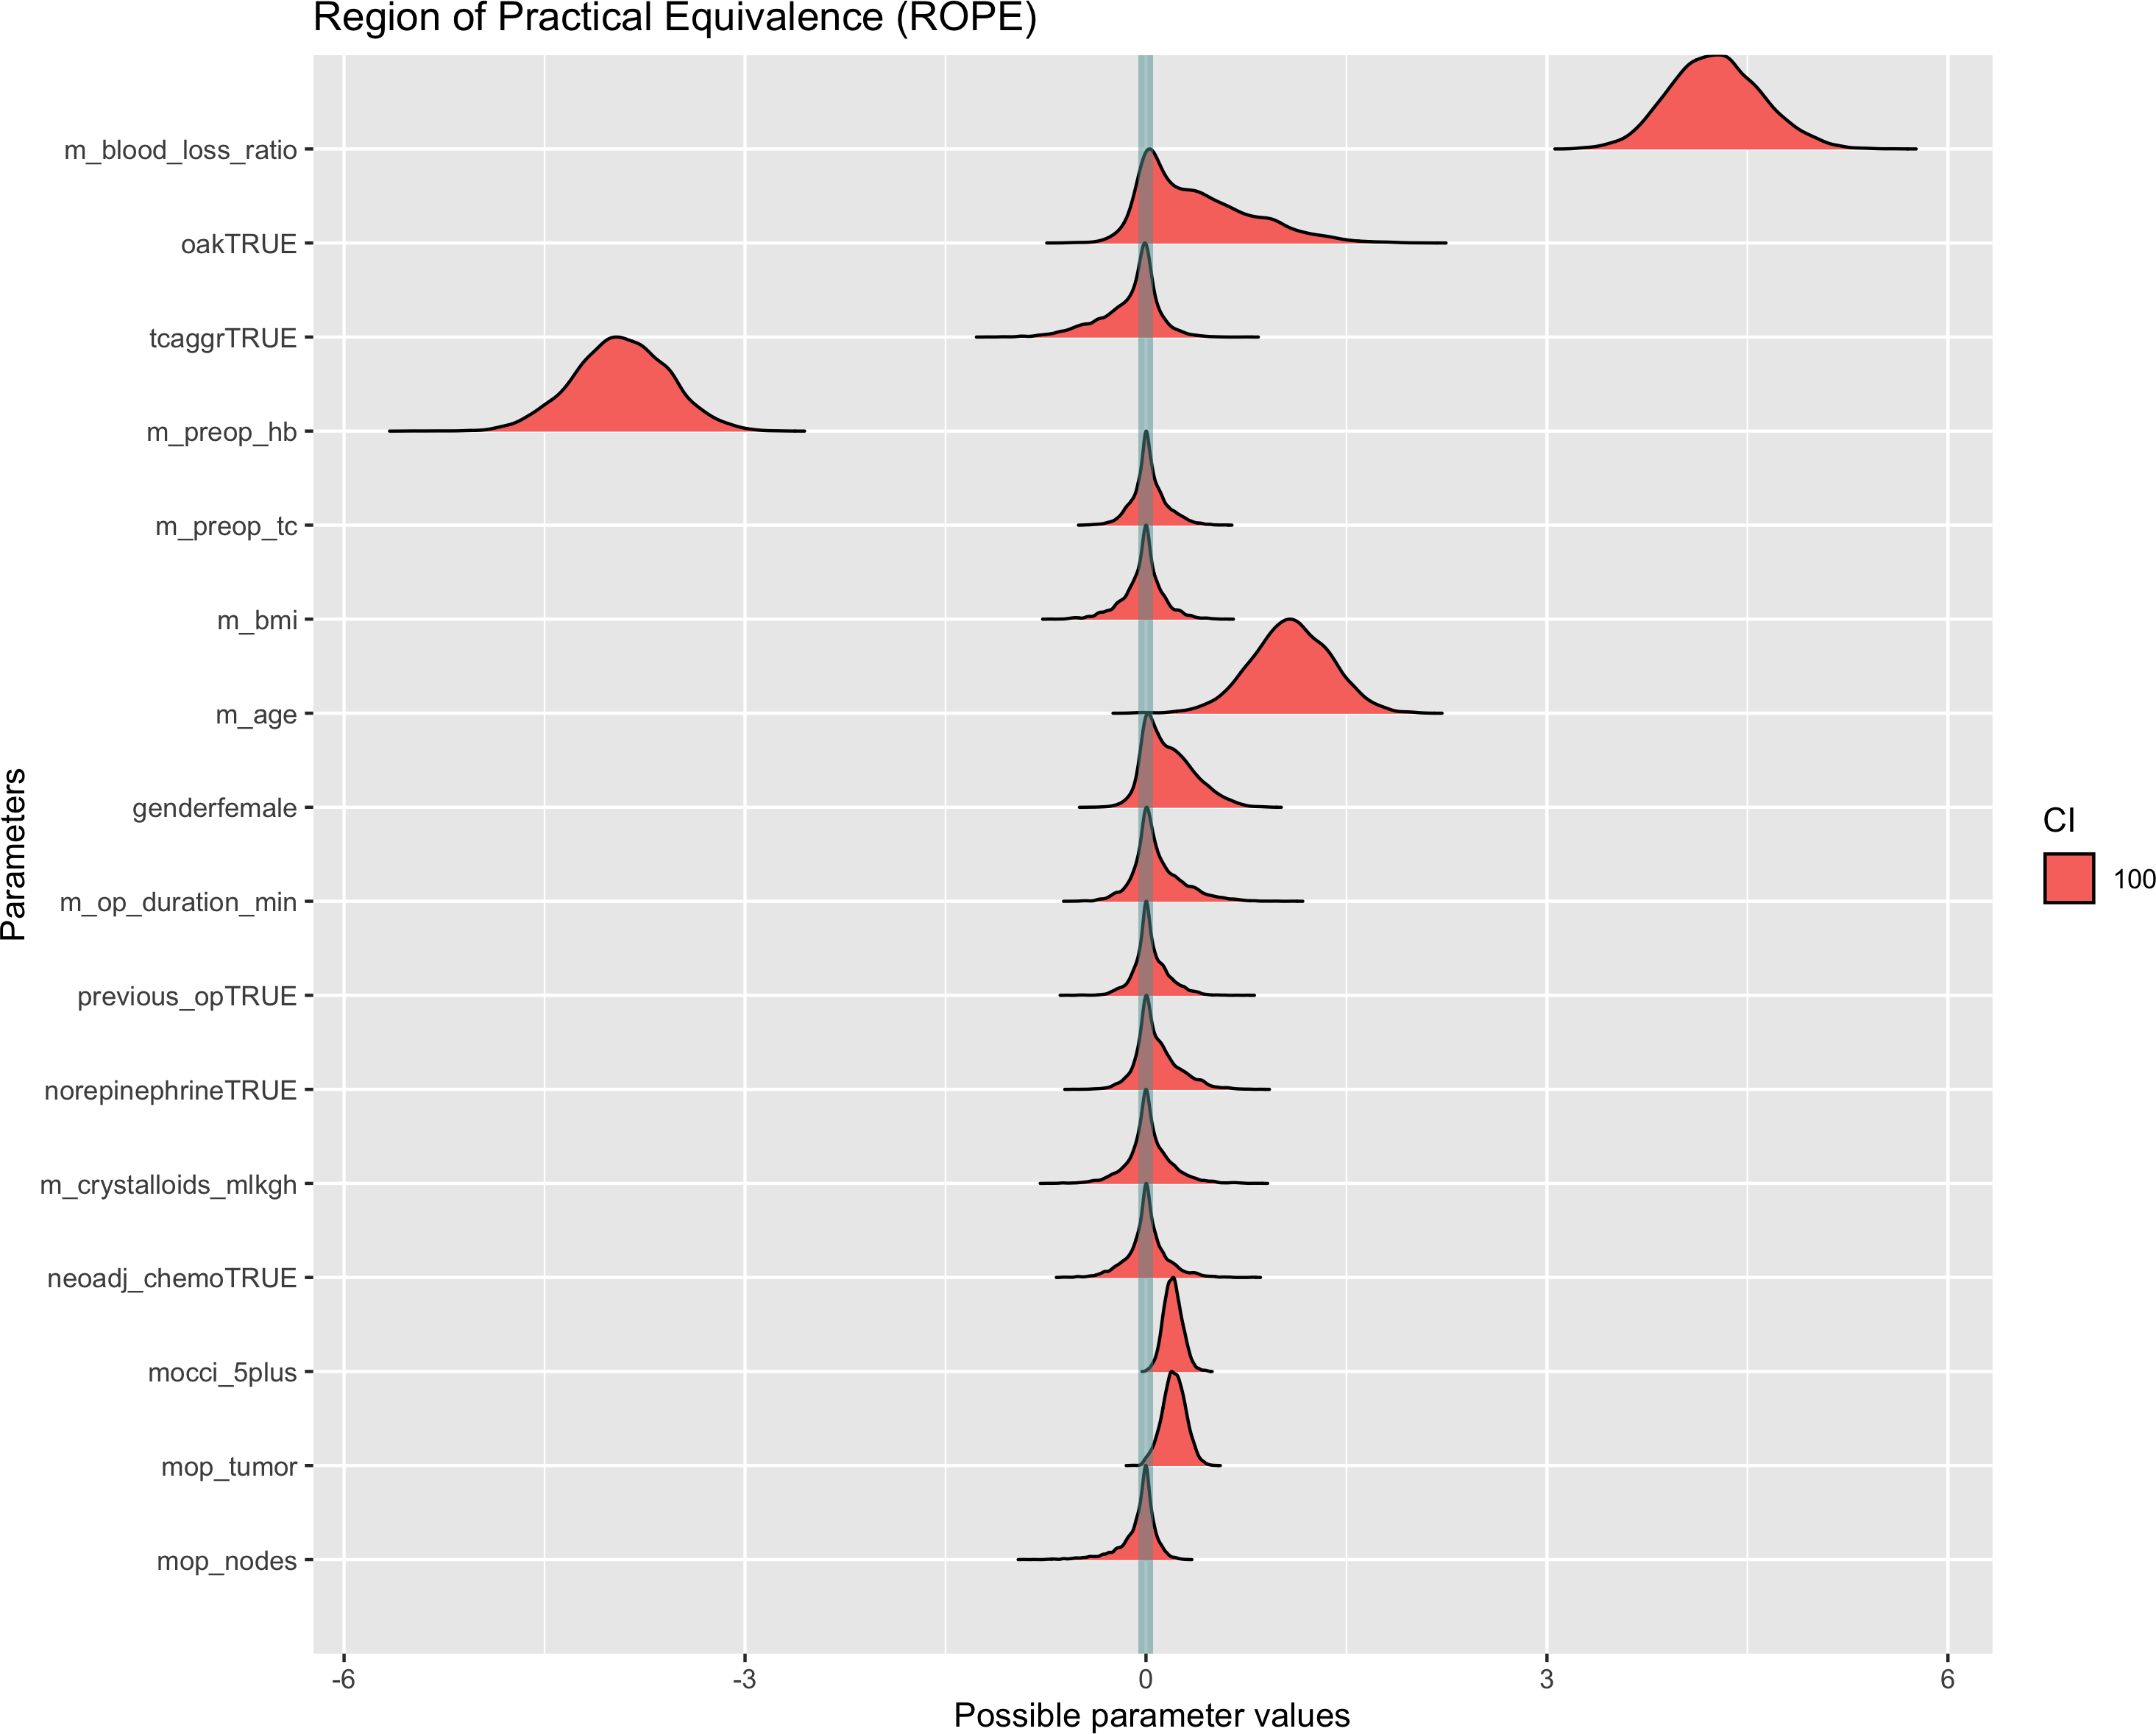
\includegraphics[width=1\linewidth]{notebook_files/figure-latex/model1full_rope-1} \end{center}

\hypertarget{roc-auc}{%
\subparagraph{ROC-AUC}\label{roc-auc}}

\begin{verbatim}
#> AUC: 0.879203428625768
\end{verbatim}

\begin{center}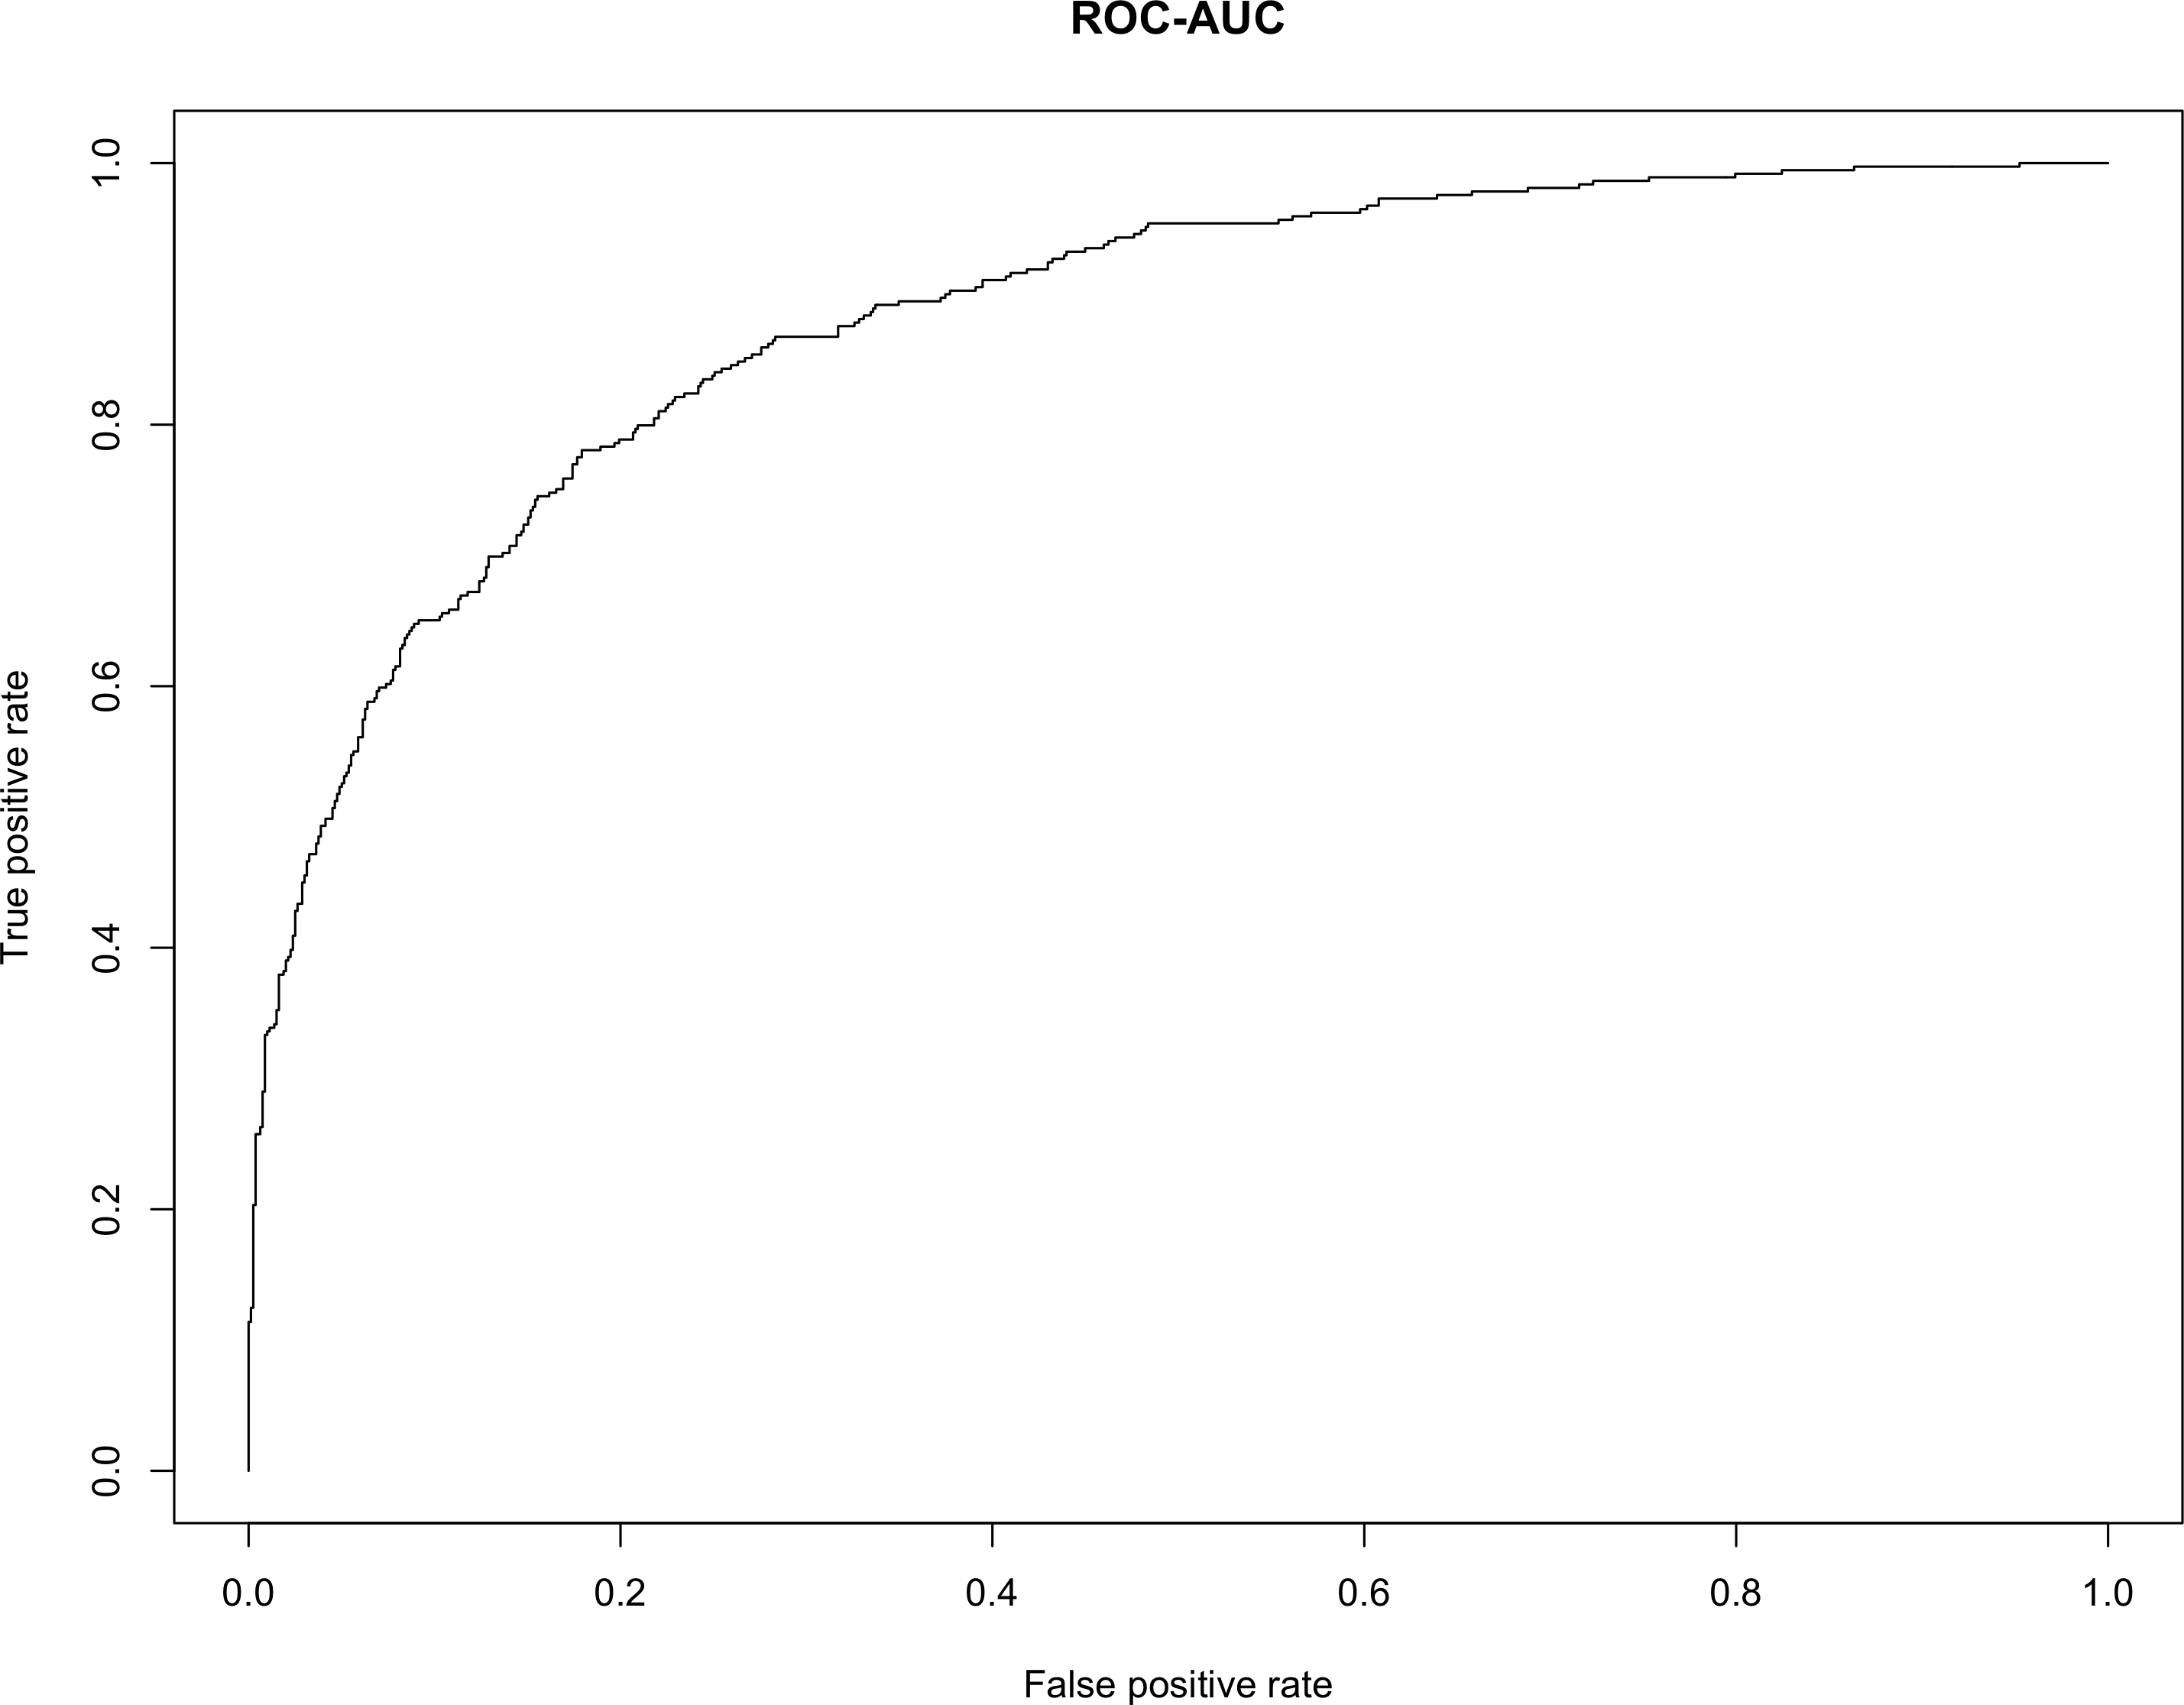
\includegraphics[width=1\linewidth]{notebook_files/figure-latex/model1full_rocauc-1} \end{center}

\hypertarget{reduced-model}{%
\paragraph{Reduced model}\label{reduced-model}}

\hypertarget{diagnostics-1}{%
\subparagraph{Diagnostics}\label{diagnostics-1}}

\begin{verbatim}
#> No divergences to plot.
\end{verbatim}

\begin{center}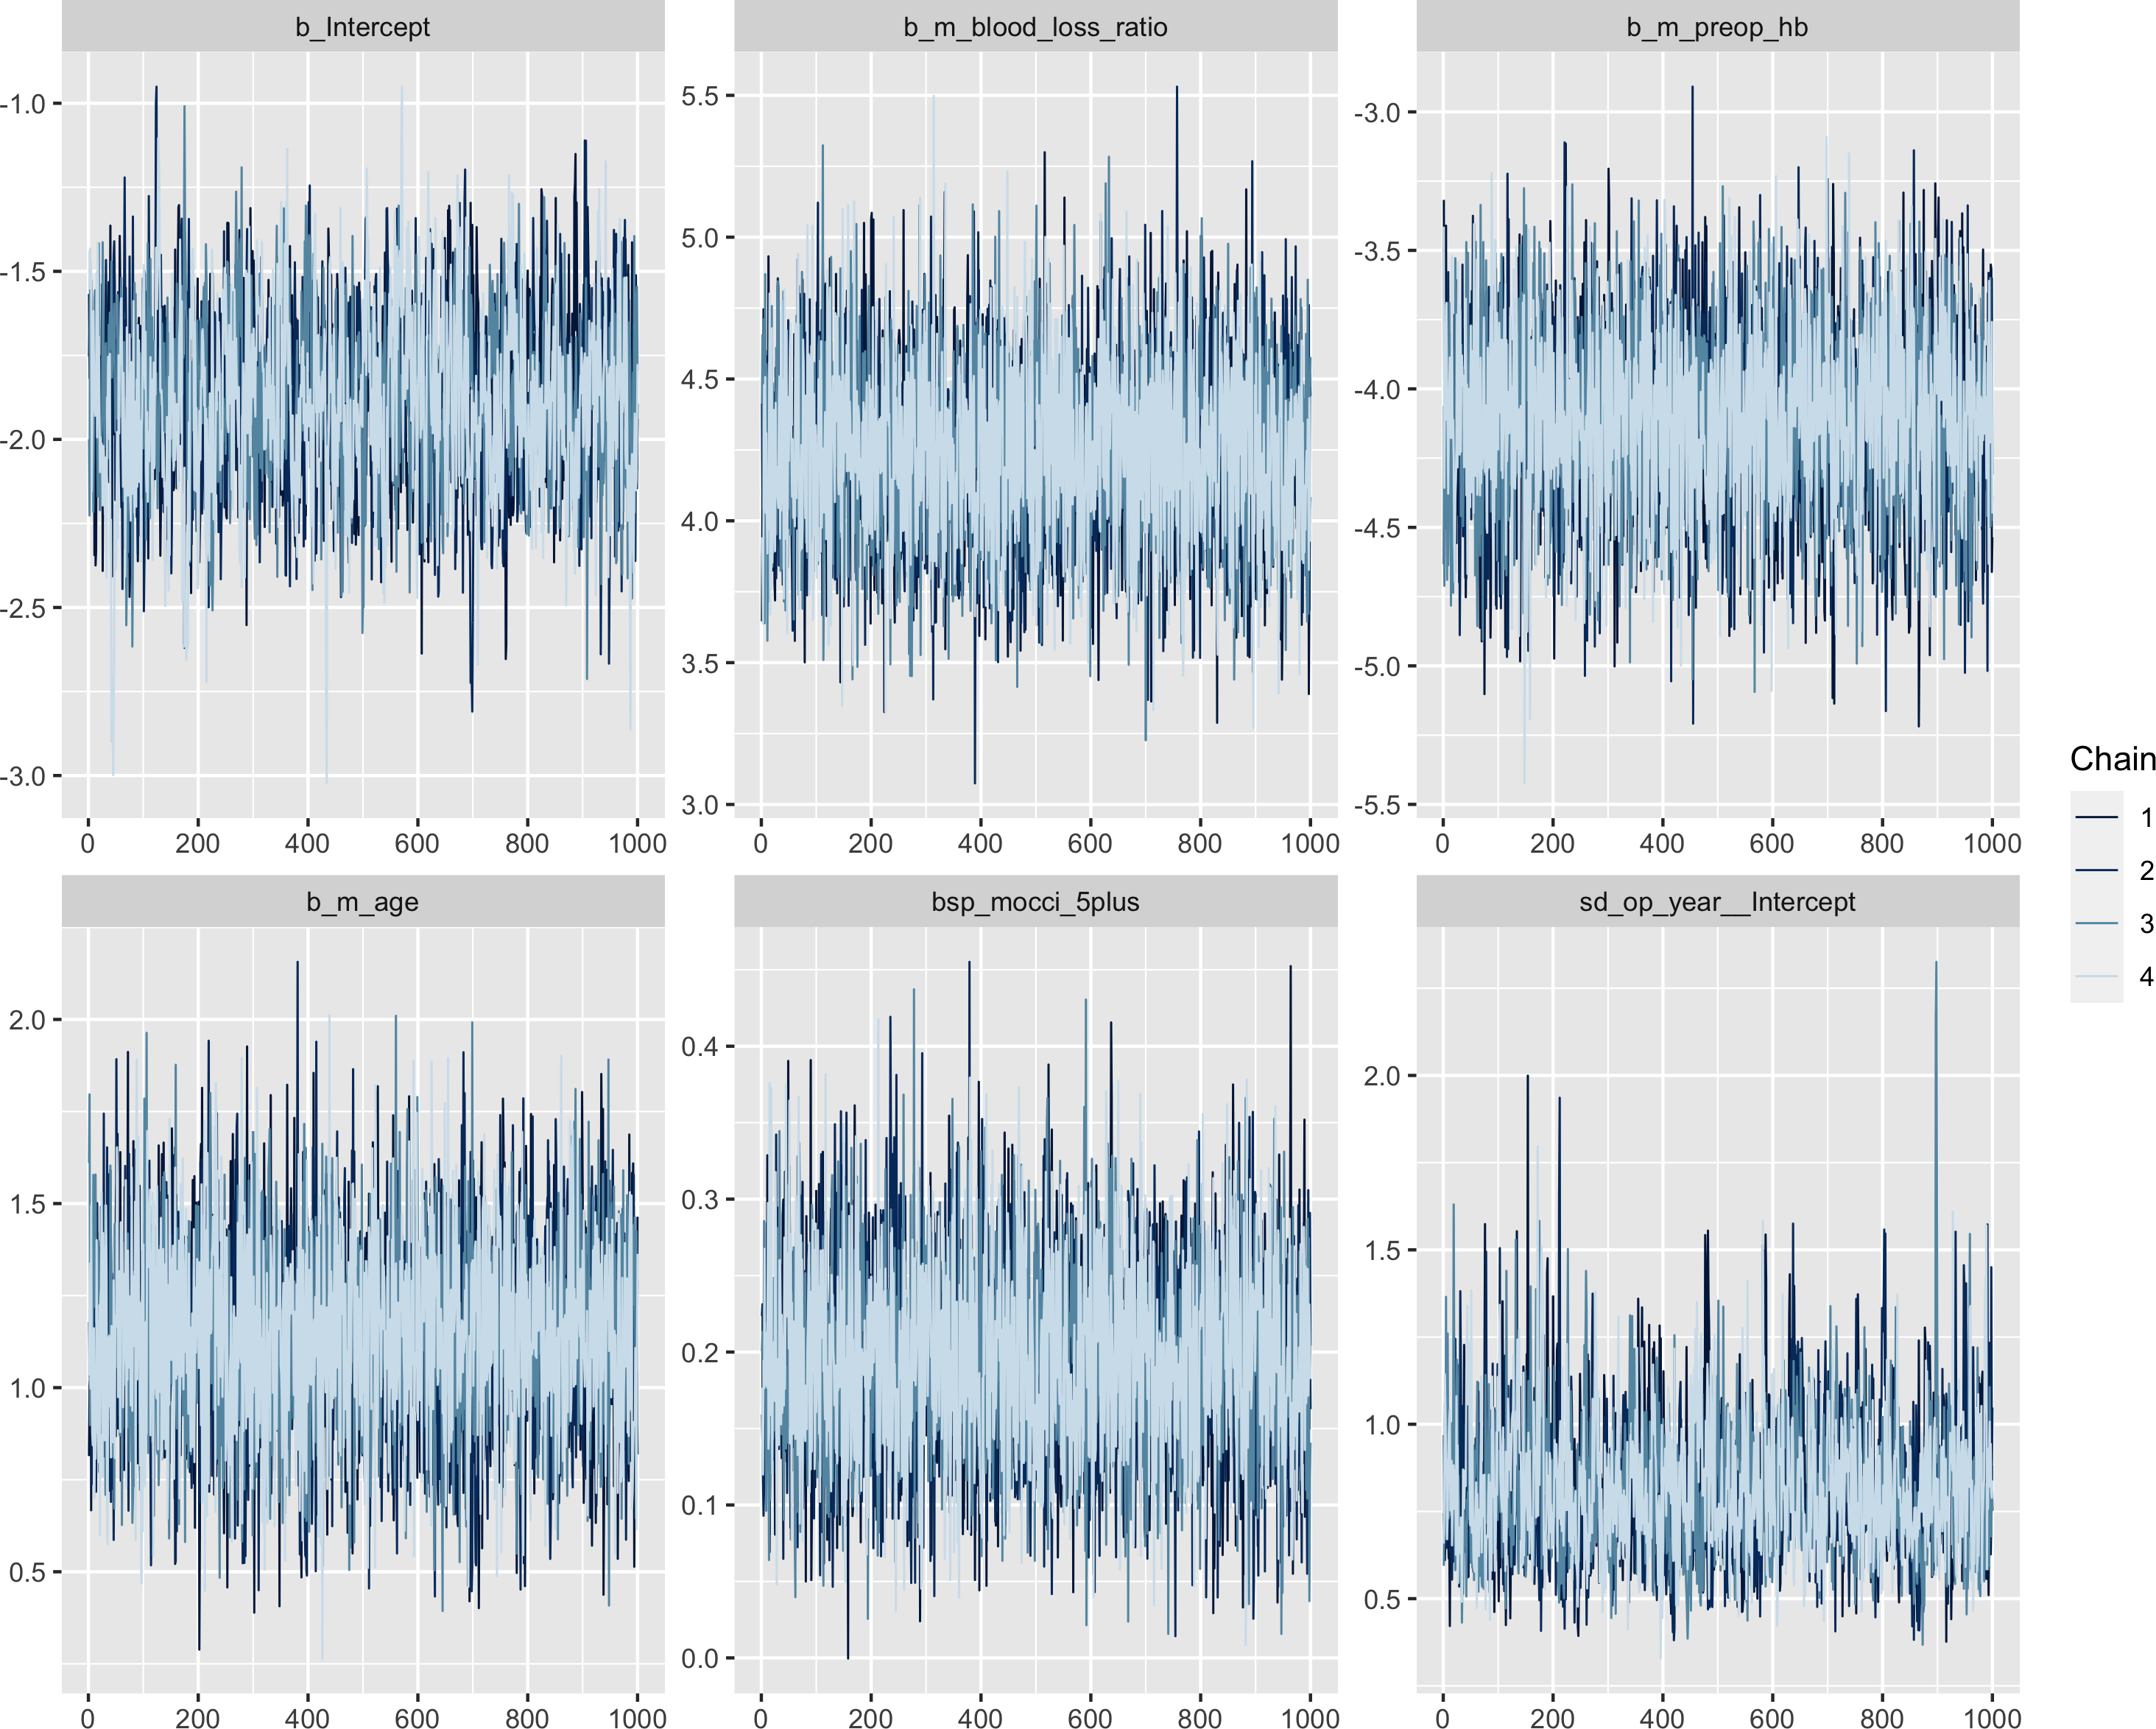
\includegraphics[width=1\linewidth]{notebook_files/figure-latex/model1reduced_diagnostics-1} \end{center}

\begin{center}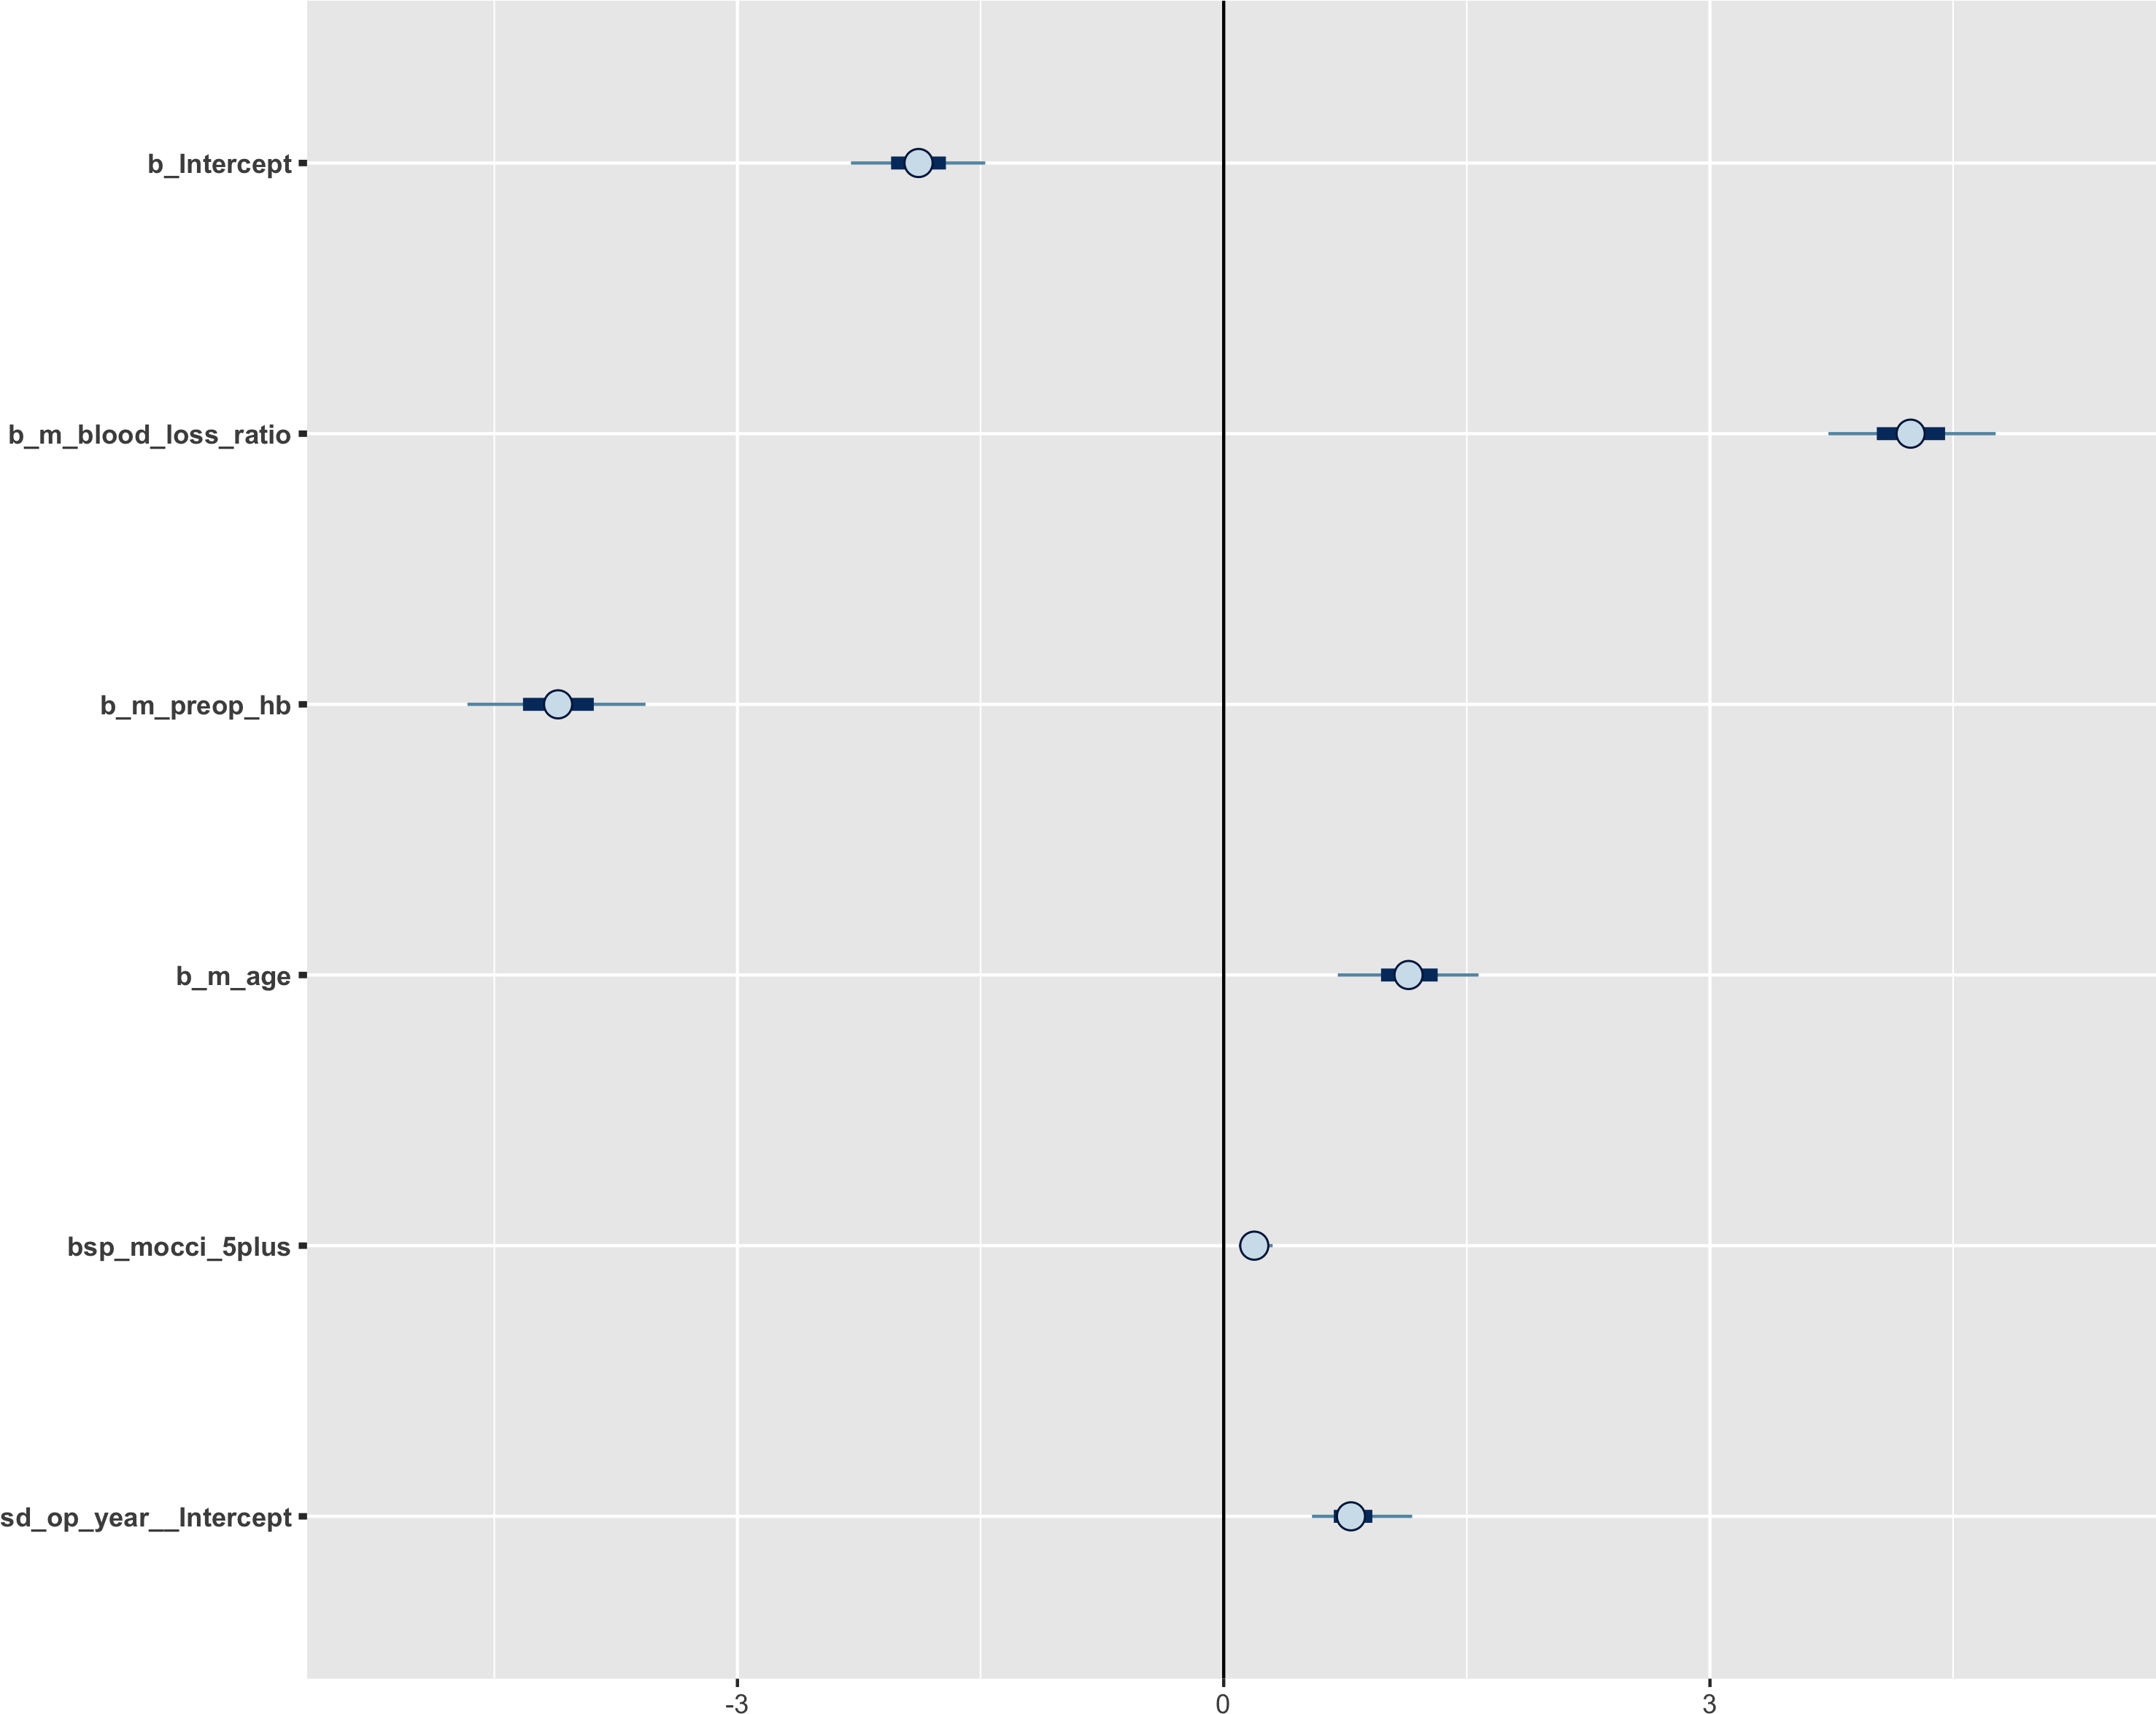
\includegraphics[width=1\linewidth]{notebook_files/figure-latex/model1reduced_diagnostics-2} \end{center}

\hypertarget{posterior-predictive-check-plot-1}{%
\subparagraph{Posterior predictive check plot}\label{posterior-predictive-check-plot-1}}

\begin{verbatim}
#> Using 10 posterior samples for ppc type 'bars' by default.
\end{verbatim}

\begin{center}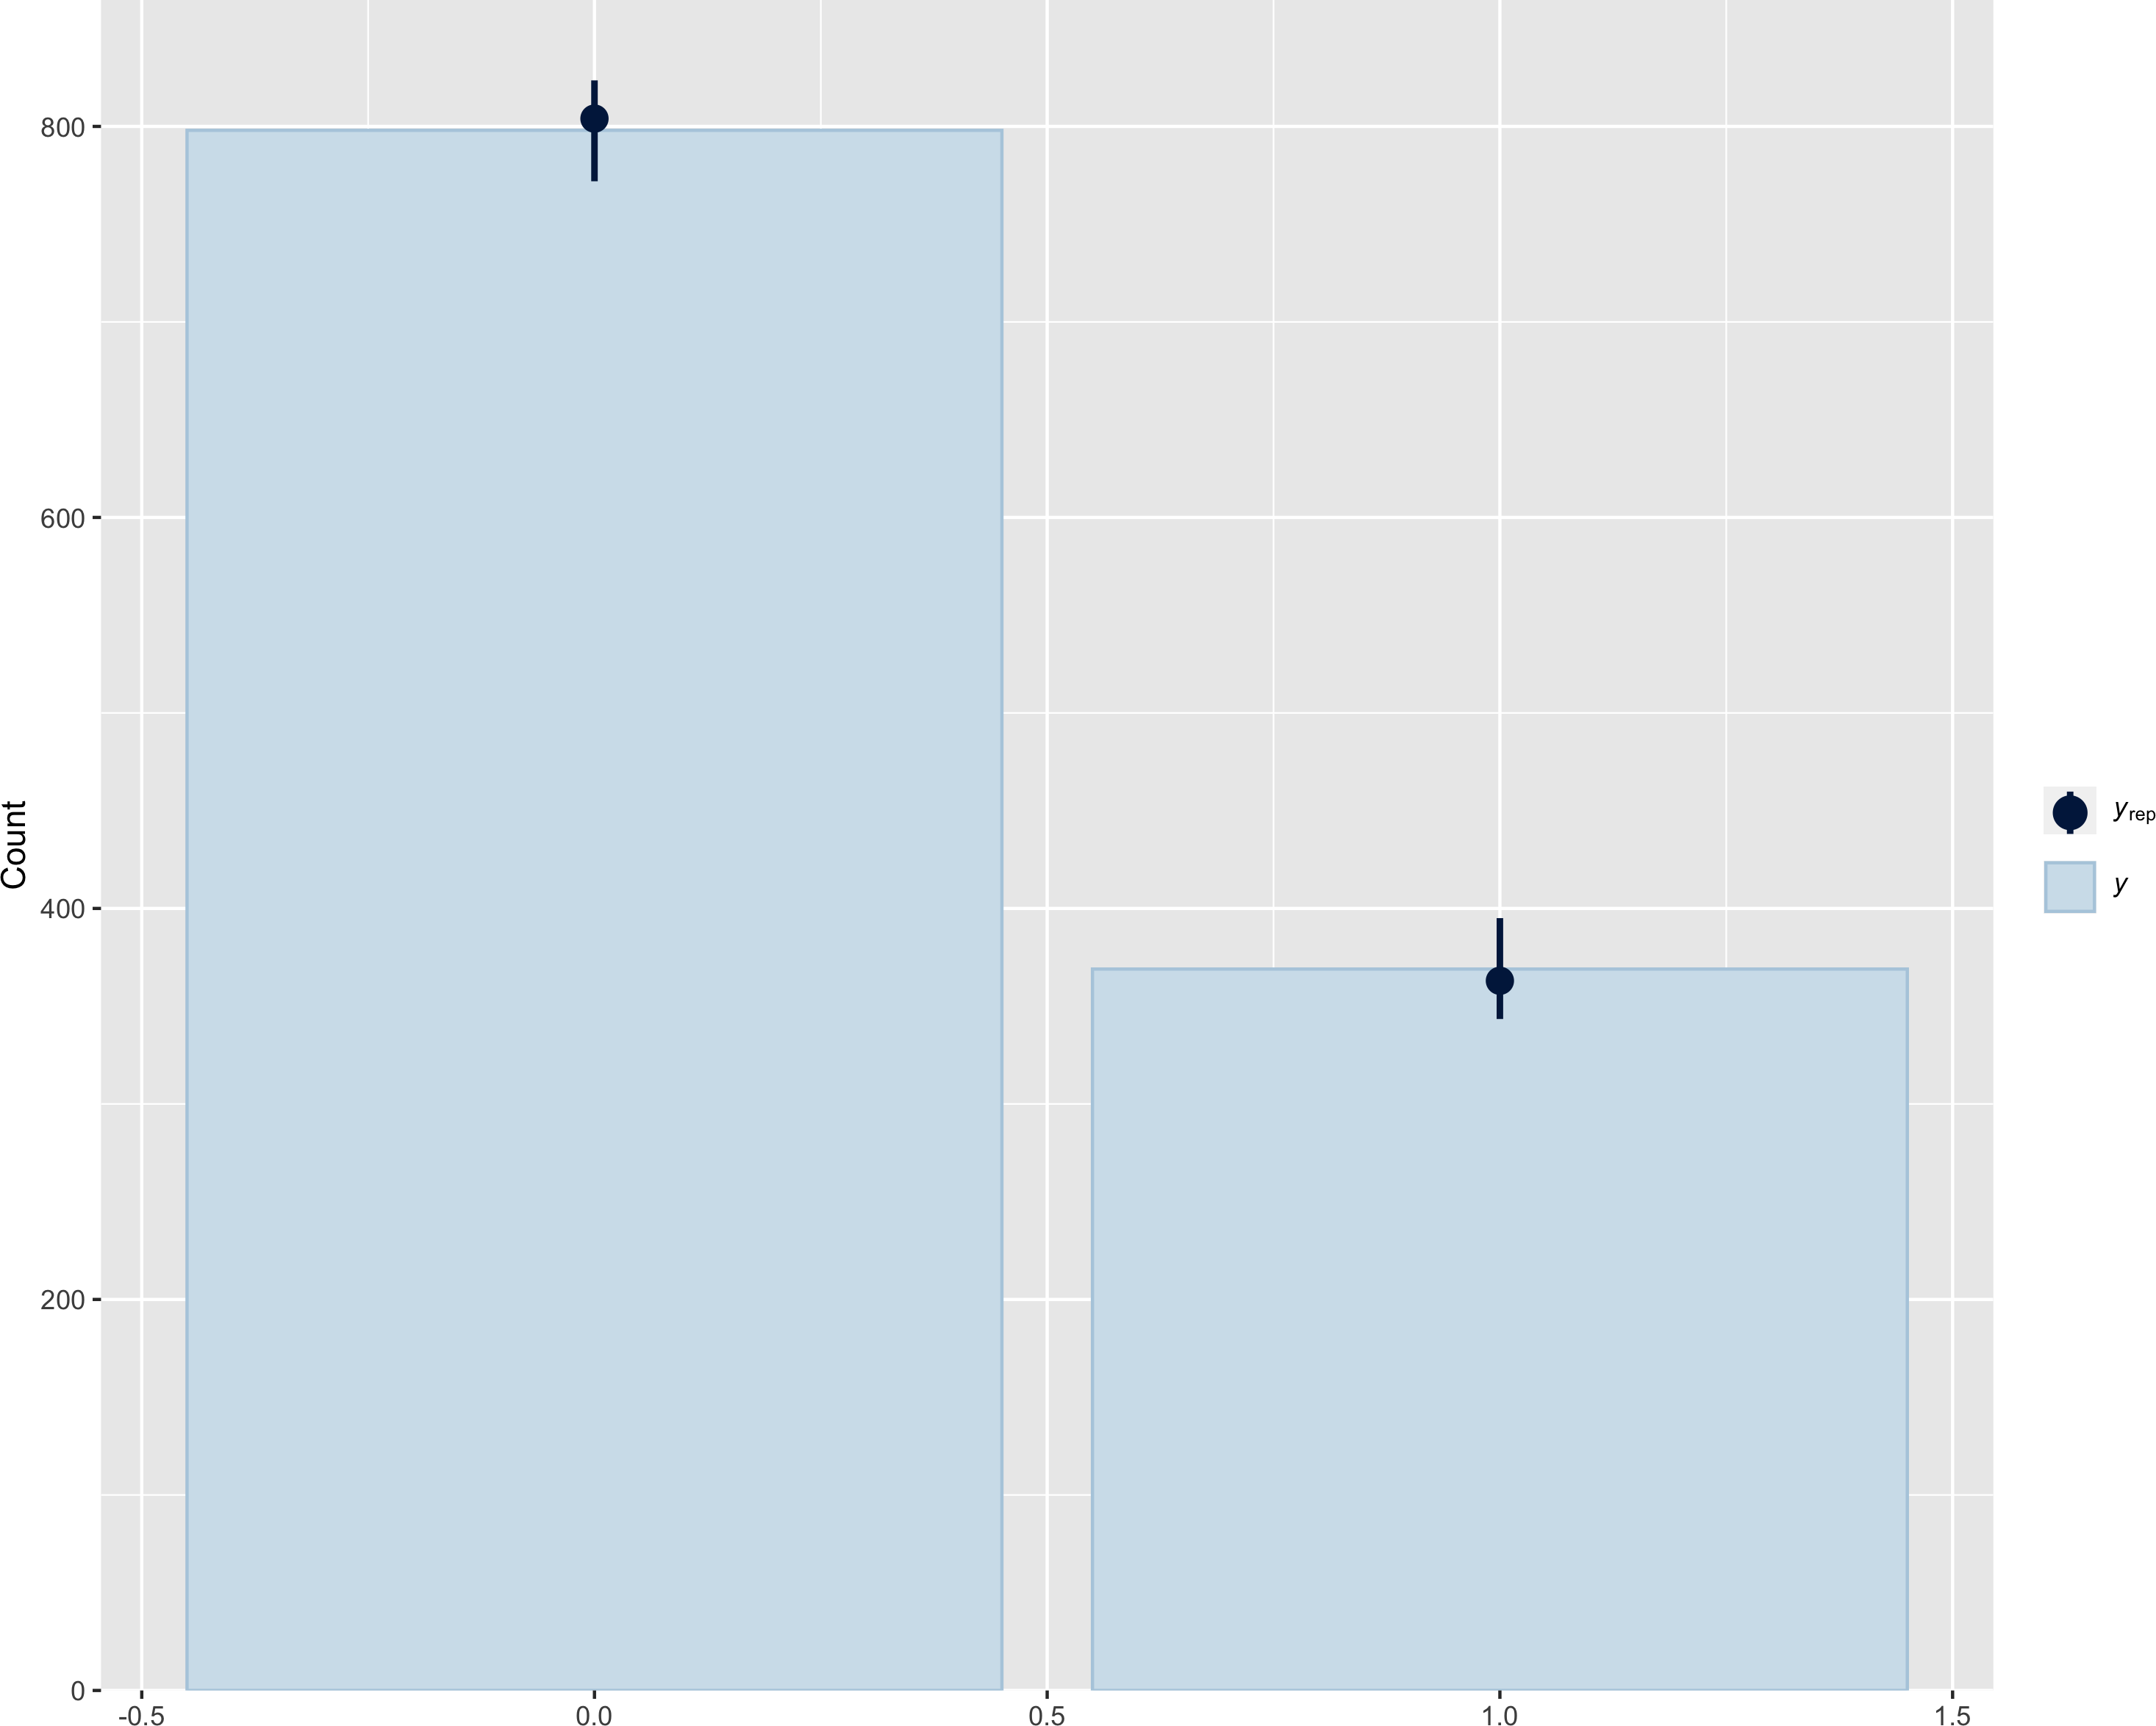
\includegraphics[width=1\linewidth]{notebook_files/figure-latex/model1reduced_ppcheck-1} \end{center}

\hypertarget{summary-1}{%
\subparagraph{Summary}\label{summary-1}}

\begin{longtable}[]{@{}ccccccc@{}}
\caption{Table continues below}\tabularnewline
\toprule
\begin{minipage}[b]{0.09\columnwidth}\centering
~\strut
\end{minipage} & \begin{minipage}[b]{0.24\columnwidth}\centering
Parameter\strut
\end{minipage} & \begin{minipage}[b]{0.09\columnwidth}\centering
Median\strut
\end{minipage} & \begin{minipage}[b]{0.05\columnwidth}\centering
CI\strut
\end{minipage} & \begin{minipage}[b]{0.10\columnwidth}\centering
CI\_low\strut
\end{minipage} & \begin{minipage}[b]{0.10\columnwidth}\centering
CI\_high\strut
\end{minipage} & \begin{minipage}[b]{0.12\columnwidth}\centering
p\_MAP\strut
\end{minipage}\tabularnewline
\midrule
\endfirsthead
\toprule
\begin{minipage}[b]{0.09\columnwidth}\centering
~\strut
\end{minipage} & \begin{minipage}[b]{0.24\columnwidth}\centering
Parameter\strut
\end{minipage} & \begin{minipage}[b]{0.09\columnwidth}\centering
Median\strut
\end{minipage} & \begin{minipage}[b]{0.05\columnwidth}\centering
CI\strut
\end{minipage} & \begin{minipage}[b]{0.10\columnwidth}\centering
CI\_low\strut
\end{minipage} & \begin{minipage}[b]{0.10\columnwidth}\centering
CI\_high\strut
\end{minipage} & \begin{minipage}[b]{0.12\columnwidth}\centering
p\_MAP\strut
\end{minipage}\tabularnewline
\midrule
\endhead
\begin{minipage}[t]{0.09\columnwidth}\centering
\textbf{1}\strut
\end{minipage} & \begin{minipage}[t]{0.24\columnwidth}\centering
b\_Intercept\strut
\end{minipage} & \begin{minipage}[t]{0.09\columnwidth}\centering
-1.916\strut
\end{minipage} & \begin{minipage}[t]{0.05\columnwidth}\centering
95\strut
\end{minipage} & \begin{minipage}[t]{0.10\columnwidth}\centering
-2.407\strut
\end{minipage} & \begin{minipage}[t]{0.10\columnwidth}\centering
-1.425\strut
\end{minipage} & \begin{minipage}[t]{0.12\columnwidth}\centering
0\strut
\end{minipage}\tabularnewline
\begin{minipage}[t]{0.09\columnwidth}\centering
\textbf{3}\strut
\end{minipage} & \begin{minipage}[t]{0.24\columnwidth}\centering
b\_m\_blood\_loss\_ratio\strut
\end{minipage} & \begin{minipage}[t]{0.09\columnwidth}\centering
4.346\strut
\end{minipage} & \begin{minipage}[t]{0.05\columnwidth}\centering
95\strut
\end{minipage} & \begin{minipage}[t]{0.10\columnwidth}\centering
3.738\strut
\end{minipage} & \begin{minipage}[t]{0.10\columnwidth}\centering
4.964\strut
\end{minipage} & \begin{minipage}[t]{0.12\columnwidth}\centering
0\strut
\end{minipage}\tabularnewline
\begin{minipage}[t]{0.09\columnwidth}\centering
\textbf{4}\strut
\end{minipage} & \begin{minipage}[t]{0.24\columnwidth}\centering
b\_m\_preop\_hb\strut
\end{minipage} & \begin{minipage}[t]{0.09\columnwidth}\centering
-4.211\strut
\end{minipage} & \begin{minipage}[t]{0.05\columnwidth}\centering
95\strut
\end{minipage} & \begin{minipage}[t]{0.10\columnwidth}\centering
-4.859\strut
\end{minipage} & \begin{minipage}[t]{0.10\columnwidth}\centering
-3.567\strut
\end{minipage} & \begin{minipage}[t]{0.12\columnwidth}\centering
0\strut
\end{minipage}\tabularnewline
\begin{minipage}[t]{0.09\columnwidth}\centering
\textbf{2}\strut
\end{minipage} & \begin{minipage}[t]{0.24\columnwidth}\centering
b\_m\_age\strut
\end{minipage} & \begin{minipage}[t]{0.09\columnwidth}\centering
1.192\strut
\end{minipage} & \begin{minipage}[t]{0.05\columnwidth}\centering
95\strut
\end{minipage} & \begin{minipage}[t]{0.10\columnwidth}\centering
0.6562\strut
\end{minipage} & \begin{minipage}[t]{0.10\columnwidth}\centering
1.711\strut
\end{minipage} & \begin{minipage}[t]{0.12\columnwidth}\centering
0\strut
\end{minipage}\tabularnewline
\begin{minipage}[t]{0.09\columnwidth}\centering
\textbf{5}\strut
\end{minipage} & \begin{minipage}[t]{0.24\columnwidth}\centering
bsp\_mocci\_5plus\strut
\end{minipage} & \begin{minipage}[t]{0.09\columnwidth}\centering
0.1941\strut
\end{minipage} & \begin{minipage}[t]{0.05\columnwidth}\centering
95\strut
\end{minipage} & \begin{minipage}[t]{0.10\columnwidth}\centering
0.08309\strut
\end{minipage} & \begin{minipage}[t]{0.10\columnwidth}\centering
0.3244\strut
\end{minipage} & \begin{minipage}[t]{0.12\columnwidth}\centering
0.004427\strut
\end{minipage}\tabularnewline
\bottomrule
\end{longtable}

\begin{longtable}[]{@{}cccccc@{}}
\toprule
\begin{minipage}[b]{0.10\columnwidth}\centering
~\strut
\end{minipage} & \begin{minipage}[b]{0.10\columnwidth}\centering
pd\strut
\end{minipage} & \begin{minipage}[b]{0.12\columnwidth}\centering
ROPE\_CI\strut
\end{minipage} & \begin{minipage}[b]{0.13\columnwidth}\centering
ROPE\_low\strut
\end{minipage} & \begin{minipage}[b]{0.14\columnwidth}\centering
ROPE\_high\strut
\end{minipage} & \begin{minipage}[b]{0.21\columnwidth}\centering
ROPE\_Percentage\strut
\end{minipage}\tabularnewline
\midrule
\endhead
\begin{minipage}[t]{0.10\columnwidth}\centering
\textbf{1}\strut
\end{minipage} & \begin{minipage}[t]{0.10\columnwidth}\centering
1\strut
\end{minipage} & \begin{minipage}[t]{0.12\columnwidth}\centering
100\strut
\end{minipage} & \begin{minipage}[t]{0.13\columnwidth}\centering
-0.055\strut
\end{minipage} & \begin{minipage}[t]{0.14\columnwidth}\centering
0.055\strut
\end{minipage} & \begin{minipage}[t]{0.21\columnwidth}\centering
0\strut
\end{minipage}\tabularnewline
\begin{minipage}[t]{0.10\columnwidth}\centering
\textbf{3}\strut
\end{minipage} & \begin{minipage}[t]{0.10\columnwidth}\centering
1\strut
\end{minipage} & \begin{minipage}[t]{0.12\columnwidth}\centering
100\strut
\end{minipage} & \begin{minipage}[t]{0.13\columnwidth}\centering
-0.055\strut
\end{minipage} & \begin{minipage}[t]{0.14\columnwidth}\centering
0.055\strut
\end{minipage} & \begin{minipage}[t]{0.21\columnwidth}\centering
0\strut
\end{minipage}\tabularnewline
\begin{minipage}[t]{0.10\columnwidth}\centering
\textbf{4}\strut
\end{minipage} & \begin{minipage}[t]{0.10\columnwidth}\centering
1\strut
\end{minipage} & \begin{minipage}[t]{0.12\columnwidth}\centering
100\strut
\end{minipage} & \begin{minipage}[t]{0.13\columnwidth}\centering
-0.055\strut
\end{minipage} & \begin{minipage}[t]{0.14\columnwidth}\centering
0.055\strut
\end{minipage} & \begin{minipage}[t]{0.21\columnwidth}\centering
0\strut
\end{minipage}\tabularnewline
\begin{minipage}[t]{0.10\columnwidth}\centering
\textbf{2}\strut
\end{minipage} & \begin{minipage}[t]{0.10\columnwidth}\centering
1\strut
\end{minipage} & \begin{minipage}[t]{0.12\columnwidth}\centering
100\strut
\end{minipage} & \begin{minipage}[t]{0.13\columnwidth}\centering
-0.055\strut
\end{minipage} & \begin{minipage}[t]{0.14\columnwidth}\centering
0.055\strut
\end{minipage} & \begin{minipage}[t]{0.21\columnwidth}\centering
0\strut
\end{minipage}\tabularnewline
\begin{minipage}[t]{0.10\columnwidth}\centering
\textbf{5}\strut
\end{minipage} & \begin{minipage}[t]{0.10\columnwidth}\centering
0.9998\strut
\end{minipage} & \begin{minipage}[t]{0.12\columnwidth}\centering
100\strut
\end{minipage} & \begin{minipage}[t]{0.13\columnwidth}\centering
-0.055\strut
\end{minipage} & \begin{minipage}[t]{0.14\columnwidth}\centering
0.055\strut
\end{minipage} & \begin{minipage}[t]{0.21\columnwidth}\centering
0.0095\strut
\end{minipage}\tabularnewline
\bottomrule
\end{longtable}

\hypertarget{region-of-practical-equivalence-1}{%
\subparagraph{Region of practical equivalence}\label{region-of-practical-equivalence-1}}

Using a ROPE range of -0.055 to 0.055 (\(0.1 \cdot \frac{\sqrt{3}}{\pi}\)) and a CI of 1.

\begin{center}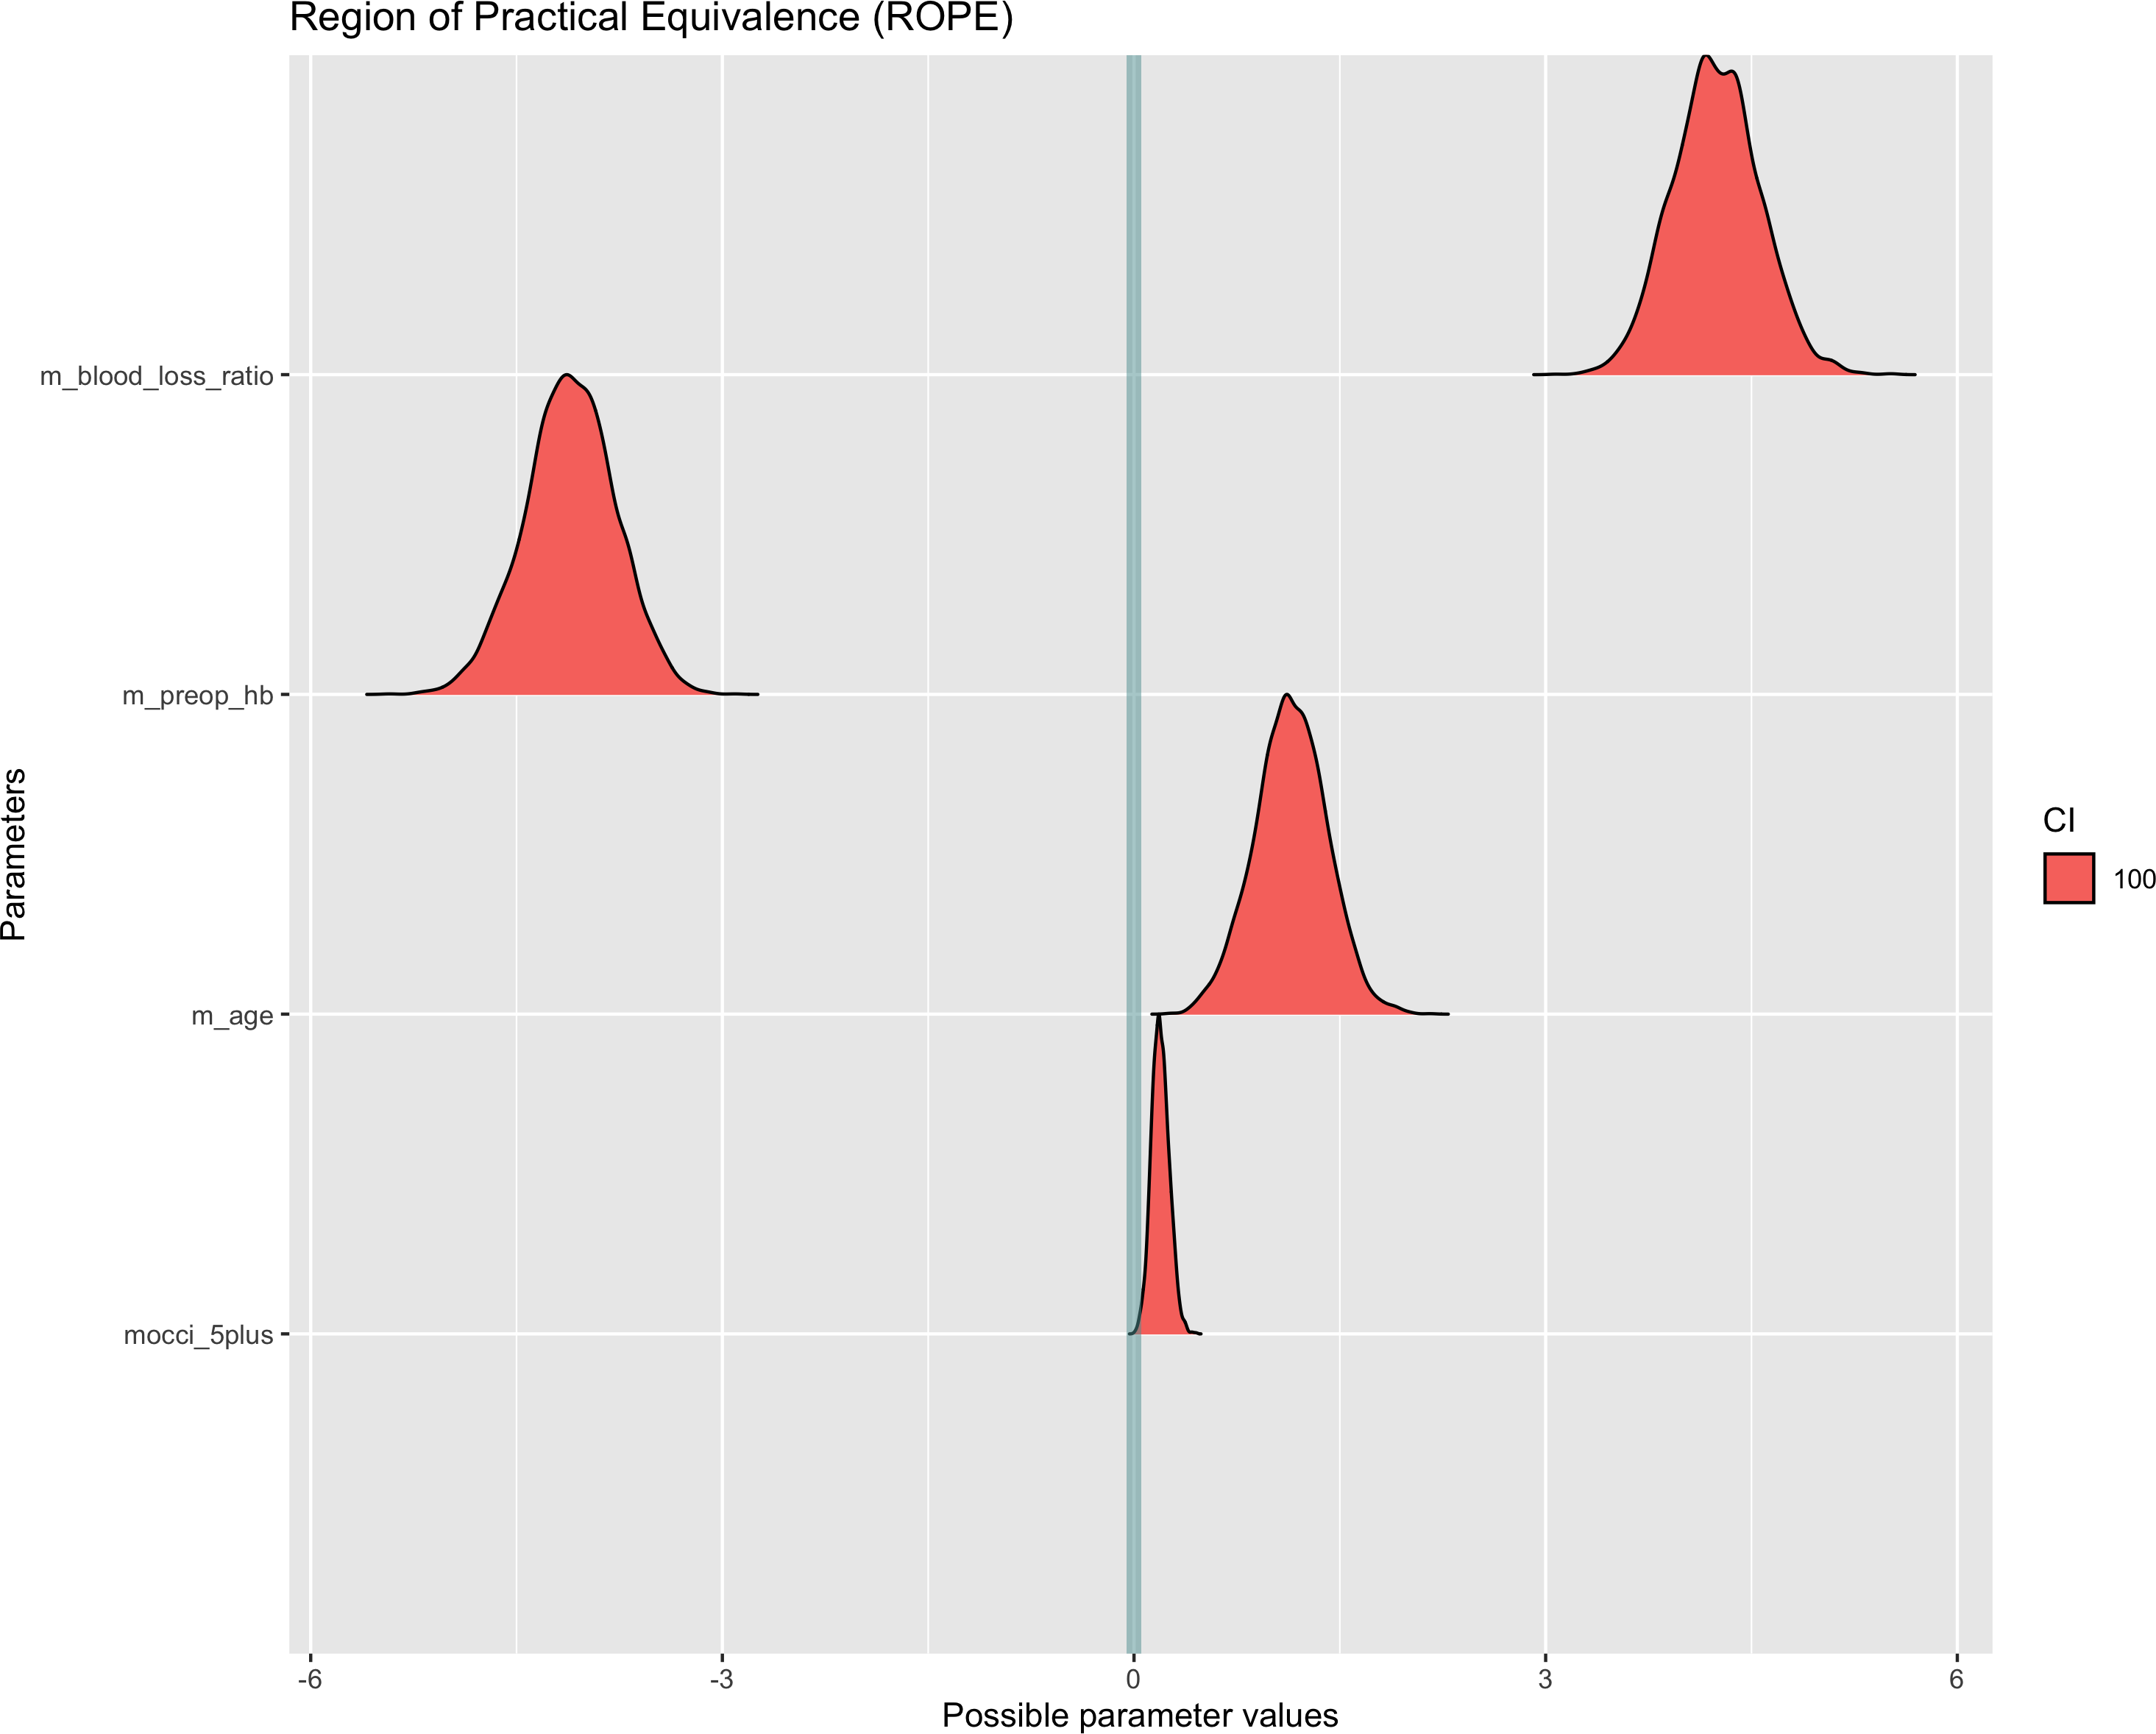
\includegraphics[width=1\linewidth]{notebook_files/figure-latex/model1reduced_rope-1} \end{center}

\hypertarget{roc-auc-1}{%
\subparagraph{ROC-AUC}\label{roc-auc-1}}

\begin{verbatim}
#> AUC: 0.873518484558283
\end{verbatim}

\begin{center}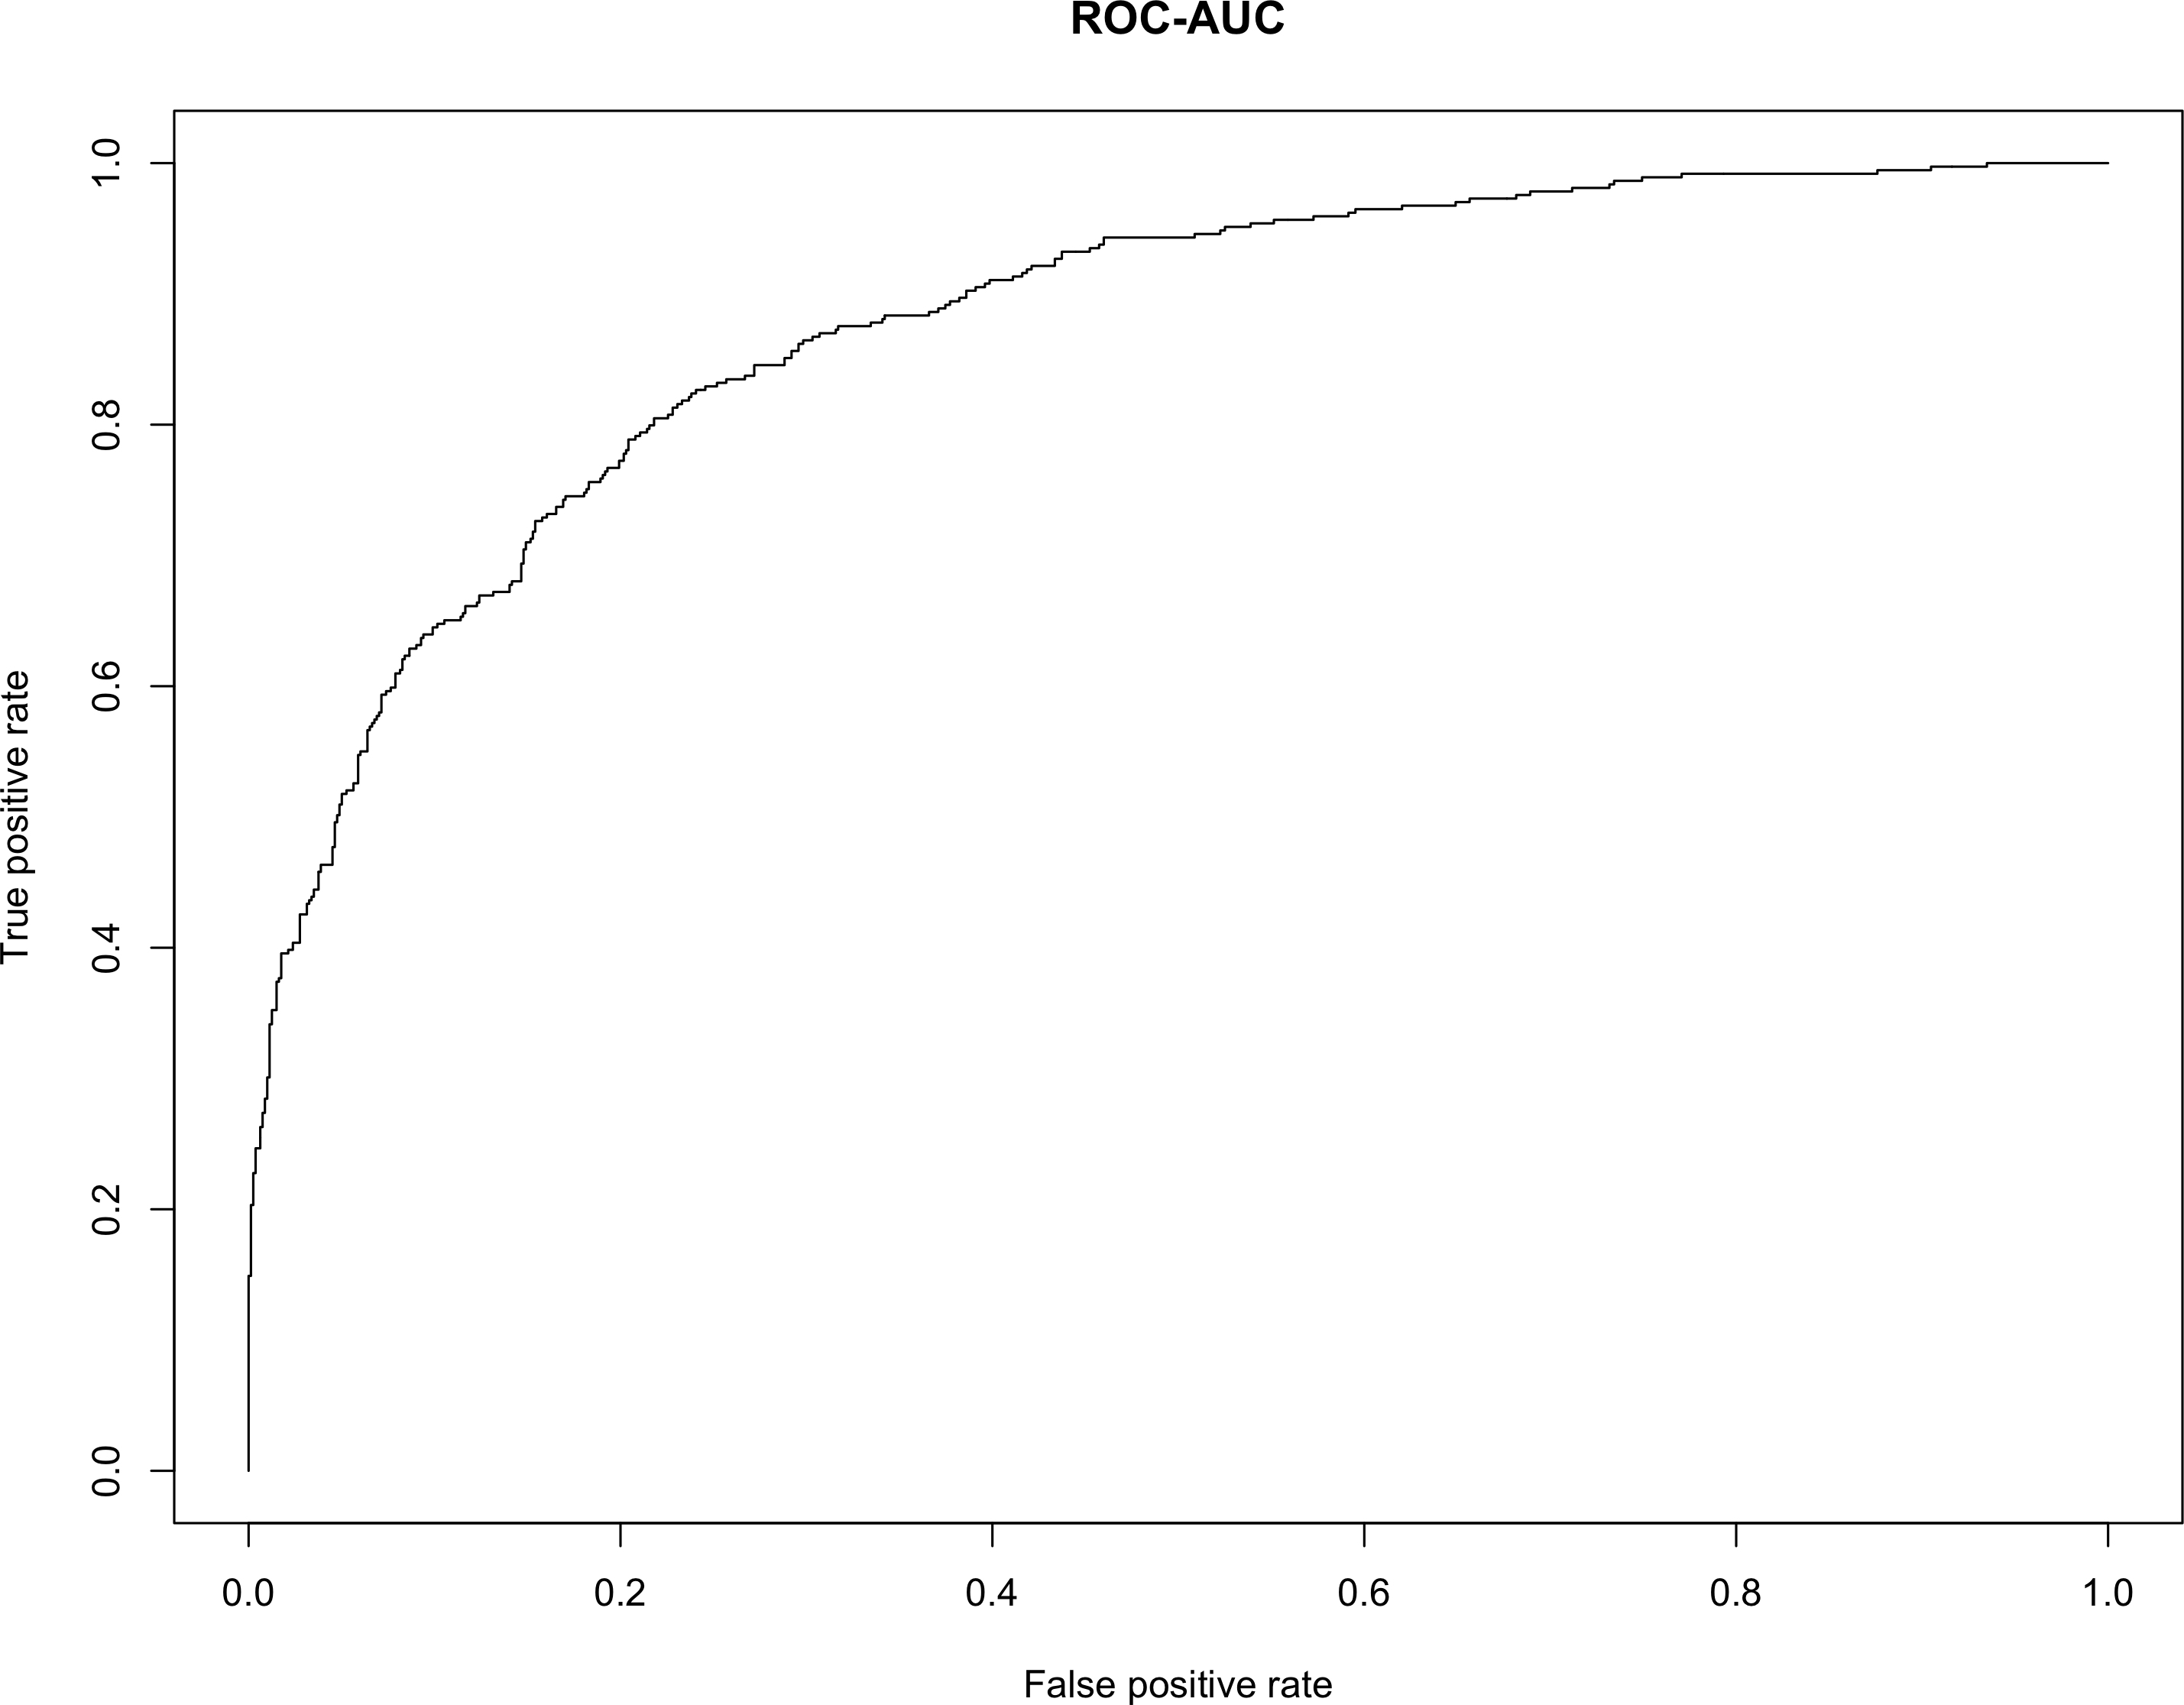
\includegraphics[width=1\linewidth]{notebook_files/figure-latex/model1reduced_rocauc-1} \end{center}

\end{document}
